\documentclass[openany,10pt,a4paper]{book}	%openany --> no blank page after each chapter / part of the book 
\setcounter{secnumdepth}{3}
 
\usepackage[utf8]{inputenc}
\usepackage{amsmath}
\usepackage{graphicx}
\usepackage[top=3cm, bottom=3cm, left=3cm, right=4cm]{geometry}

\usepackage[T1]{fontenc}

\usepackage{wrapfig}

\usepackage{pdfpages}

\usepackage{tikz}

\usepackage{fancyhdr}
	\lhead{  OCULAR }%OCuLAR - Online objeCt LeArning & Recognition}
	\chead[]{}
	\rhead[]{Page \thepage }
	\cfoot{}


\setlength{\headsep}{1.5cm}
	\pagestyle{fancy}

%%algunos símbolos matemáticos y paquete para usar subimágenes
%\usepackage{amsmath}
%\usepackage{amsfonts}
%\usepackage{amssymb}
%\usepackage{graphicx}
%\usepackage{subfigure}
%\usepackage{listings}
%\usepackage{appendix}

%Hyperrefs without borders
\usepackage[hidelinks]{hyperref}

%reset the numbering each part
\makeatletter
\@addtoreset{chapter}{part}
\makeatother  

%parametros del documento (sus propiedades)
\hypersetup{
    pdftitle={ OCULAR - In-hand object recognition and on-line learning using 2D and 3D information },
    pdfsubject={Bachelor's Thesis - 2014},
    pdfauthor={Irene Sanz Nieto},
    pdfkeywords={palabraclave1} {palabraclave2} {palabraclave3},
    colorlinks,
    citecolor=black,
    filecolor=black,
    linkcolor=black,
    urlcolor=black,
}

\usepackage{indentfirst} 

\begin{document}

%Elements that appear before the thesis itself
\frontmatter

%cada incluye referencia a un archivo de tipo .tex
\begin{titlepage}
\begin{center}

%forma de introducir imágenes. el \\[0.5 cm] de final de línea introduce un salto de ese tamaño.
%width=1\textwidth indica el tamaño de la imágen (valores entre 0-1). 
 
\includegraphics[size=0.8]{img/uc3m.eps}  \\[0.5 cm]

\large \textsc{Automated Systems Engineering Department} \\ [1 cm]

\large Bachelor's Thesis\\[1 cm]

\huge \textsc{In-hand on-line object recognition and learning using 2D and 3D information}\\[13 cm]


%flushleft alinea a la izquierda el texto
\begin{flushleft} \Large
\emph{Author:} Irene Sanz Nieto\\[0.5 cm]
\emph{Supervisor:} Víctor González Pacheco \\

\end{flushleft}

%rellena de blanco el resto de la página para escribir abajo del todo
\vfill

% Bottom of the page
{\large Madrid, June 2014}

\end{center}
\end{titlepage}


%\include{licencia}

%\include{evaluacion}


\chapter*{Acknowledgements}
    
\begin {center}

\end{center}

I would like to thank my boyfriend Alvaro for his support and comprehension during the whole project and for his help and patience in the difficult moments. 
\\

I wish to acknowledge my parents as well. They have always supported and encouraged me. They teached me the importance of learning and also the importance of always giving the best possible version of oneself.
\\

I also would like to thank the teachers I had during my life. Those who were better for helping me to easily acquire the knowledge of their subjects, and those who were worse for aiding me in learning how to overcome difficulties and be self-sufficient. 
\\


I am particularly grateful for the assistance given by my thesis supervisor, Víctor González Pacheco, for teaching me how to make rigorous documentation and how to organize a project correctly. Also, for giving me some key pointers without which this project would not have been possible. 
\\
  
And finally, I would like to thank my friends and family, specially Rocío and Blanca for being always there. 



%\include{resumen}


%%%%%% TABLE OF CONTENTS %%%%%%
\tableofcontents

%%%%%% TABLE OF FIGURES %%%%%%
\listoffigures


%%%%%% DESCRIPTIVE PART %%%%%%
\mainmatter

%%% INTRODUCTION
\addcontentsline{toc}{chapter}{Introduction}
\chapter*{Introduction}

% Intro

This bachelor's thesis consists on a software that implements an in-hand object learning and recognition using 2D and 3D information. 
\\

The code was designed to be running inside a robot. Hence, everything is modularized and all processes are designed to run in parallel. 

The hardware needed for this project is an RGB-D sensor and a computer. 

\addcontentsline{toc}{section}{What does the software do?}
\section*{What does the software do?}
% What does it do?
The input of the software is the image and the point cloud provided by the RGB-D sensor. The output of the system is different depending on the mode we are working. If the user is making it learn a new object, the output is the percentage of learning completed. On the other hand, if the user is utilizing the recognizing mode, the output of the system is the identifier of the object, i.e. the number that represents which object in the dataset seems to be more similar to the one being shown to it currently. 

%%%%%%%%%%%%%%%%%%%%%%%%%%%%%%%%%%PICTURE

\addcontentsline{toc}{section}{How can it be used?}
\section*{How can it be used?}
% How it is used?
From the beginning, a easy and intuitive human-machine interface was a must. In order to achieve this, this simple state 
machine was designed:

%%%%%%%%%%%%%%%%%%%%%%%%%%%%%%%%%%%%%PICTURE

The software only allows one hand being used at a time. It will select the hand that is located highest. 

In order to switch between the learning and recognizing modes of the program, the distance between the hand and the body
is being used: 

If the hand is stretched out towards the RGB-D sensor, the software will start learning. If it is closer to the body, 
it will launch the recognizing mode, which is the default. 

\addcontentsline{toc}{section}{General characteristics of the software}
\section*{General characteristics of the software}
% How is the code coded?

The Robotic Operating System is being used in this project since it has numerous features that allow a more efficient and 
easier implementation of software that has the characteristics described above. More information about this operating 
system may be found in the section.
%%%%%%%%%%%%%%%%%%%%%%%%%%(!!!!SECTION).

The software developed in this thesis is a ROS package. The last release might be downloaded from the following link. 
%%%%%%%%%%%%%%%%%%%%%%%%%%%%%%%%LINK


\addcontentsline{toc}{section}{Thesis structure}
\section*{ Thesis structure}

%motivation: 
	%contexto
	%problem
	%intro de la solución 
	
	
	


%%% STATE OF THE ART
%%\addcontentsline{toc}{part}{State of the art}
\part{State of the art}

\addcontentsline{toc}{chapter}{Introduction}
\chapter*{Introduction}

% Intro

This bachelor's thesis consists on a software that implements an in-hand object learning and recognition using 2D and 3D information. 
\\

The code was designed to be running inside a robot. Hence, everything is modularized and all processes are designed to run in parallel. 

The hardware needed for this project is an RGB-D sensor and a computer. 

\addcontentsline{toc}{section}{What does the software do?}
\section*{What does the software do?}
% What does it do?
The input of the software is the image and the point cloud provided by the RGB-D sensor. The output of the system is different depending on the mode we are working. If the user is making it learn a new object, the output is the percentage of learning completed. On the other hand, if the user is utilizing the recognizing mode, the output of the system is the identifier of the object, i.e. the number that represents which object in the dataset seems to be more similar to the one being shown to it currently. 

%%%%%%%%%%%%%%%%%%%%%%%%%%%%%%%%%%PICTURE

\addcontentsline{toc}{section}{How can it be used?}
\section*{How can it be used?}
% How it is used?
From the beginning, a easy and intuitive human-machine interface was a must. In order to achieve this, this simple state 
machine was designed:

%%%%%%%%%%%%%%%%%%%%%%%%%%%%%%%%%%%%%PICTURE

The software only allows one hand being used at a time. It will select the hand that is located highest. 

In order to switch between the learning and recognizing modes of the program, the distance between the hand and the body
is being used: 

If the hand is stretched out towards the RGB-D sensor, the software will start learning. If it is closer to the body, 
it will launch the recognizing mode, which is the default. 

\addcontentsline{toc}{section}{General characteristics of the software}
\section*{General characteristics of the software}
% How is the code coded?

The Robotic Operating System is being used in this project since it has numerous features that allow a more efficient and 
easier implementation of software that has the characteristics described above. More information about this operating 
system may be found in the section.
%%%%%%%%%%%%%%%%%%%%%%%%%%(!!!!SECTION).

The software developed in this thesis is a ROS package. The last release might be downloaded from the following link. 
%%%%%%%%%%%%%%%%%%%%%%%%%%%%%%%%LINK


\addcontentsline{toc}{section}{Thesis structure}
\section*{ Thesis structure}

\section{Hardware }
This section shows the hardware specifications with which the testing was performed. 

\subsection{Computer}

\subsection{RGB-D sensor}


\newpage
\section{Object learning and recognition}

Object learning and recognition is an active field. 
In this section the most important works related to that field are presented. 
Also, the differences and improvements performed in this thesis with respect to the previous art are stated. 
% In this section the most important works related to this thesis are exposed. 

\subsection{Object learning and recognition using 2D and 3D input data}

This special branch in the object learning and recognition field has been active for many years. 
One of the first works in the field was the one performed by D.M.Gavrila and F.C.A. Groen. 
In 1992,  they developed a  system that performs 3D object recognition using 2D input data \cite{D.M.Gavrila1991}.
A 3D model was created and then the new 2D projection was matched to this model.
A geometric hashing method of matching was applied to the input 2D projection. 
The image was only matched to a model if the error to a nearby 2D projection was within certain thresholds.
The testing was performed under a controlled environment and using textured objects. 
The system would not give the same results in a real environment with noise and loosely defined objects. 
Also, the use of hashing limits the size of the dataset due to its high computing cost. 
\\

Later systems as \cite{Sheta2012} explore different descriptors for the objects that result less time-consuming. 
In this case, fuzzy logic is used to match the learned features to the new ones. 
Those descriptors are a set that include Affine \cite{Reiss:1991:RFT:117668.117680}, Zemike \cite{Teague} and Hu \cite{Hu1962} moments invariants among others. 
The results obtained a high percentage of true positives. 
But, again, the system uses a controlled setup:
The input is collected from three cameras that has a known illumination and orientation. 
The objects are white with significantly different shapes and they rest in a black background during learning and recognition phases. 
The applications in which it could be used are more related to the industrial field than the robotics field. 
\\

An outdoor system is described in \cite{Zia2013}, which demonstrated the effectiveness of two methods when combined: local descriptors and 3D wireframes. 
The system was able to distinguish between cars and bicycles and to estimate their pose. 
The input of the recognition is a single 2D image. 
Nevertheless, the training was made off-line, using a high number of Computer-Aided Design (CAD) model's views. 
\\

These systems differ with the one presented in this thesis in one major aspect: 
the user-software interaction. 
This thesis is based on providing an easy and intuitive interface. 
The learning process is performed easily and on-line and the recognition is real-time. 
There is no setting needed, no previous processing and care about the environment. 
The combination of 2D and 3D information in my system is, to the best of my knowledge, unique. 
The fact of recognizing the objects using those two different methods and then apply a decision algorithm better the results, reducing the effect of the noise.  



\subsection{In-hand object learning and recognition}

Most of the literature in object learning and recognition has been developed using wearable cameras as the input of the system. 
One of the most representative works is \cite{Roth2006}, which consists in a camera used to capture daily objects to construct a dataset more easily. 
Its main feature is that it eliminates the necessity of manually segmenting and labeling the learning datasets for object recognition libraries. 
It only learns new templates that are later fed to a off-line learning algorithm. 
\\

Another example is \cite{Philipose2009}, in which a benchmarking of an egocentric object recognition system is performed. 
This in-hand object recognition uses as input an image that has the object used at the center. 
The background is not segmented in this system because the errors produced by it may be neglected.
The object occupies most of the camera's frame and hence the processing of the input data to the system does not need to be as exhaustive as the one developed in this thesis.  
\\

The system presented here has a different approach: an in-hand object recognition and learning in which the user is located in front of the acquisition device. 
It is a solution to the same problem, the recognition of an object that a user holds, but the initial setting is different. 
In my thesis, the user is in front of the camera, because the software is running on a robot. 
The interaction between the software and the user is different from the previous art on the field. 
This change in the input creates an additional difficulty due to the hand's segmentation in the input image. 
\\

Furthermore, to the best of my knowledge there is no previous art in in-hand object learning and recognition using 2D and 3D information combined together. 
All of the algorithms described in this section use a camera and hence 2D data as input. 
The inclusion of 3D and the independence between the 2D and 3D recognition processes improve the noise resistance of my system with respect to the previous art. 


% \paragraph{Template matching}


% In the object recognition field obtaining good descriptors is of paramount importance. 
% The quality of the features extracted as the model of the object determine the quality of the algorithm. 
% Due to this importance, the next chapter is devoted to the descriptors that can be obtained from 2D and 3D data.




%%%%%%%%%%%%%%%%%%%%%%%%%%%%% 				DESCRIPTORS 				%%%%%%%%%%%%%%%%%%%%%%%%%%%%%%%%%%%%%%%%%%55


\section{Feature Extraction algorithms}
In chapter \ref{fundamentals} a brief introduction to the characteristics of the different feature extractor algorithms was performed. 
In this section the different state-of-the-art algorithms for 2D and 3D feature extraction are presented and compared. 

\subsection{Algorithms for 2D Feature Extraction}
\label{2d_features}


The most used algorithms for general object recognition are presented in this section. 
% due to their relation between performance, invariantness and speed are exposed below. 
They appear in chronological order and the differences, similarities and improvements between them are explained. 
The selection of one algorithm or another depends on the application.


\paragraph{SIFT}\mbox{}\\
\label{sift}

SIFT (Scale Invariant Feature Transform) is a scale and rotation invariant feature descriptor \cite{sift}. 
There are various papers in which the performance of SIFT is compared with other descriptors and one of the most representative is \cite{Mikolajczyk2005}. In it, it can be seen that SIFT 
outperforms the previous algorithms, mainly due to its combination of local information and relative strengths and orientations of gradients. This combination makes it more robust to illumination and viewpoint changes and to noise. 
\\

The SIFT algorithm is based on four main phases: 
The first step is to detect the scale-space extrema, i.e. the location of potential interest points that are invariant to scale and rotation. 
The next step is to test those potential keypoints and select the more relevant based on measures of their stability. 
Then, one or more orientations are assigned to each of the previously obtained keypoints based on local image gradient directions. 
The following operations are performed on data that has been transformed relative to the location, scale and orientation of these features. 
This grants the invariantness to these transformations. 
The final phase consists on the description of the selected keypoint transforming the local image gradients into a representation that is descriptive enough to permit the information of various levels of shape distortion and illumination change. 
\\

In order to minimize the cost of extracting such a distinctive features, a cascade filtering approach is used in order to apply the most time-consuming operations only at locations that pass an initial test. 
It can be used for on-line applications but it still has a latency that was later improved. 
In order to reduce that lag, there were different approaches previous to the apparition of algorithms such as ORB, that reduced it drastically \cite{orb}. 
As an example, in \cite{sift_fpga} the SIFT algorithm was implemented on a FPGA (Field Programmable Gate Array), improving its speed by an order of magnitude and thus allowing it to run in real-time.
\\

The main reason of the high computing time of SIFT features is the descriptor vector size. 
In the aim of creating a highly distinctive descriptor, the vector is over-dimensioned slowing the detection, description and matching processes. 
This over-dimension is patent in the duplication of information that could be removed without affecting in a high degree its descriptiveness. 
% In relation with object recognition, this algorithm has a good performance in medium cluttered spaces. If the image is cluttered, there will appear a number of features of the background that do not have a match in the given database. Hence, it will give false positives and the match will have a lower probability. 




\paragraph{SURF}\mbox{}\\

SURF (Speeded Up Robust Features) is a scale and rotation invariant interest point or keypoint detector and descriptor \cite{surf}. 
It is a proprietary algorithm that simplifies the detection, extraction of the descriptors and matching steps thus obtaining them much faster than previous algorithms without losing repeatability, distinctiveness or robustness. 
\\

SURF algorithm is composed of three main steps: 
The first step of the algorithm is to identify the interest points such as corners, blobs or T-junctions, i.e. a junction were two lines meet forming a T. 
Therefore, this algorithm will be useful when evaluating a textured object.
The next step is to represent the neighbourhood of the interest points as a feature vector. 
The final step is to match the descriptor vectors between different images, in order to stablish a recognition of a pattern. Usually the matching is performed using as a reference the distance between the vectors. 
In this part, it can be perceived that the size of the descriptor vectors affects directly the performance of the algorithm. SURF aims to reduce that size without losing distinctiveness in the features. 
\\
\newpage
The SURF algorithm appeared after SIFT and hence it is interesting to see the similarities and differences between the two. 
In section \ref{descriptors} it was seen the good results obtained when combining the local information and relative data regarding gradients. This algorithm is based on similar characteristics: 
First, an orientation based on the information extracted from a circular region with the interest point as its center is obtained. Then, a square region aligned to that orientation is described and the descriptor is extracted from it.  
\\

The experiments in \cite{surf} show that the performance of these descriptors equals and in some cases improves the one of the SIFT descriptors. Also, the SURF descriptors are much faster computed and matched due to its smaller size. 


\paragraph{ORB}\mbox{}\\

ORB (Oriented FAST and Rotated BRIEF) is a fast rotation invariant, noise resistant binary descriptor based on BRIEF \cite{orb}.
ORB authors claim that it is two orders of magnitude faster than SIFT while matching its performance in many situations. 
Nevertheless, since ORB is not scale invariant, if the scale difference is noticeable the SURF algorithm will outperform ORB. 
\\

The features used in ORB build on the Features from Accelerated Segment Test (FAST) \cite{fast} keypoint detector and the Binary Robust Independent Elementary Features (BRIEF) \cite{brief} descriptor. Both of this previous algorithms offer a good performance and computing time relation. Since neither of them had the orientation taken into account, the main improvement made by the ORB developers is to include this feature in the algorithm. Also, the computation of oriented BRIEF features was improved and an analysis of variance and correlation for this features created. 
\\

FAST is mainly used to find keypoints in real-time systems that match visual features. The orientation operator included in this algorithm is the centroid operator described in \cite{orientation_corners}. This technique is not computationally demanding and also, unlike SIFT, it returns a single dominant result. 
\\

BRIEF uses simple binary tests whose performance is similar to SIFT with regard to robustness to lighting, blur and perspective distortion, but it is sensitive to in-plane rotation. In order to eliminate this drawback, the lowest computing costing solution is to steer BRIEF accordingly with the orientation of the keypoints. 
\\

In the different tests in \cite{orb} can be seen that the percentage of inliers obtained with ORB are higher and do not variate as much as those obtained by SIFT or SURF. 
ORB is then a good alternative for the latter if the application does not need a scale invariant descriptor. 
Finally, it is noticeable that this algorithm is Open Source.
Both SIFT and SURF are patent protected and the use for research is permitted, but for commercial uses the payment of a fee is needed. % is since the previous ones are proprietary. 
For all the above reasons, the ORB algorithm is the one being used in the system developed in this thesis. 


\subsection{Algorithms for 3D Feature Extraction}
\label{3d_features}


Applied to 3D data, a feature is a characteristic that describes a point inside the data. Features or descriptors can be compared to determine whether the point described is the same in two different inputs. They are used in object recognition and there are many different descriptors that can be used. Each of them has a certain speed in its computing and a reliability and robustness associated.
\\

Depending on the application in which they appear the developer must select the features depending on the specifications. 
As an example, two geometric point features are the underlying surface's estimated curvature and the normal at a specific query point. 
Both are local features and they characterize the point using the information provided by its neighbors. 
There are two types of features: local and global. 
Local features are less time-expensive but they are less robust. 
This means that two different objects may obtain very similar local features.
Global descriptors implement different techniques to generalize the information obtained for keypoints or important points in the mesh. 
They take more time to compute but are more robust than the previous ones. 
Since in our application the speed is key, local features are being used. 
\\

There exist a number of 3D local features that are computed using combinations of different geometric characteristics of the points. 
As an example, the 3D SIFT descriptor \cite{Scovanner2007} is obtained performing the 3D gradient and magnitude for each pixel, which is directly derived from its computation in 2D. 
It is rotation and scale invariant but is very time-consuming. 
The 3D descriptors being used in this thesis are the Point Feature Histogram (PFH) features. 

\subsubsection{Point Feature Histogram (PFH)}
\label{pfh}

The Point Feature Histogram \cite{Rusu2008} is a local 3D descriptor. 
It is fast to compute but its level of detail is limited. 
They are computed approximating the geometry of a point's k-neighborhood with a few values. 
This fact results in the possibility of obtaining a similar set of points in a very different object. 
\\

The PFH descriptors are invariant to rotation, position and point cloud density. 
They also perform well with noisy data. 
The features are created representing the mean curvature around the query point using a histogram of values. 
The normals' direction and magnitude of the points in the k-neighborhood of that point are studied. 
\\

The Fast Point Feature Histogram (FPFH) \cite{Rusu} descriptor is also a local descriptor based in the PFH. 
It is faster because it considers only the direct relations between the query point and its neighbors.
This fact makes them less robust than the previous descriptors. 
This is the reason why the Point Feature Histogram descriptors are the ones being used in this thesis instead of the Fast Point Feature Histogram descriptors. 






%%% SYSTEM DESCRIPTION
%\addcontentsline{toc}{part}{System Description}
\chapter{System Description}
\label{system_description}

\addcontentsline{toc}{chapter}{Introduction}
\chapter*{Introduction}

% Intro

This bachelor's thesis consists on a software that implements an in-hand object learning and recognition using 2D and 3D information. 
\\

The code was designed to be running inside a robot. Hence, everything is modularized and all processes are designed to run in parallel. 

The hardware needed for this project is an RGB-D sensor and a computer. 

\addcontentsline{toc}{section}{What does the software do?}
\section*{What does the software do?}
% What does it do?
The input of the software is the image and the point cloud provided by the RGB-D sensor. The output of the system is different depending on the mode we are working. If the user is making it learn a new object, the output is the percentage of learning completed. On the other hand, if the user is utilizing the recognizing mode, the output of the system is the identifier of the object, i.e. the number that represents which object in the dataset seems to be more similar to the one being shown to it currently. 

%%%%%%%%%%%%%%%%%%%%%%%%%%%%%%%%%%PICTURE

\addcontentsline{toc}{section}{How can it be used?}
\section*{How can it be used?}
% How it is used?
From the beginning, a easy and intuitive human-machine interface was a must. In order to achieve this, this simple state 
machine was designed:

%%%%%%%%%%%%%%%%%%%%%%%%%%%%%%%%%%%%%PICTURE

The software only allows one hand being used at a time. It will select the hand that is located highest. 

In order to switch between the learning and recognizing modes of the program, the distance between the hand and the body
is being used: 

If the hand is stretched out towards the RGB-D sensor, the software will start learning. If it is closer to the body, 
it will launch the recognizing mode, which is the default. 

\addcontentsline{toc}{section}{General characteristics of the software}
\section*{General characteristics of the software}
% How is the code coded?

The Robotic Operating System is being used in this project since it has numerous features that allow a more efficient and 
easier implementation of software that has the characteristics described above. More information about this operating 
system may be found in the section.
%%%%%%%%%%%%%%%%%%%%%%%%%%(!!!!SECTION).

The software developed in this thesis is a ROS package. The last release might be downloaded from the following link. 
%%%%%%%%%%%%%%%%%%%%%%%%%%%%%%%%LINK


\addcontentsline{toc}{section}{Thesis structure}
\section*{ Thesis structure}

\newpage
\section{Design alternatives}
% In the present section the steps that were taken in order to obtain the final system for solving the problem are presented. 
This section presents the steps that were taken to obtain the final system. 
% The intermediate designs are analyzed and their pros and cons evaluated. 
The different intermediate designs are shown and the reasons behind the change from one to another are explained. 
The final design can be found in section \ref{system_design}.
\\

\paragraph{First design}
\mbox{} \\

The first design was based in using a hardware with low cost and high accessibility, a camera. The decision of including that device forced the input information to be two-dimensional. The C++ programming language was selected for its high performance and the OpenCV library was picked to aid in the data processing. It was seen that the two dimensional information was not sufficient to obtain a reliable hand tracking. Also, this task created a high lag due to the high amount of computing it needed. 
\\


\paragraph{Hand tracking problem}
\mbox{} \\

In order to reduce the time spent in the hand tracking, it was decided to take advantage of the 3D capabilities of the RGB-D sensors. 
In this case, a Kinect is used, which is a low cost device. 
%The fact of having the information of the absolute position of the points in the space gave the new possibility of segmenting using the depth parameter. 
This type of sensors return a point cloud, a data matrix that presents the objects in front of it using three-dimensional information. 
This fact allowed to segment the scene using the depth parameter, reducing the amount of data that needed processing. 
\\

At this point, it was necessary to create a hand-tracker before starting the project itself, that is, the object learning and recognition nodes. 
Also, the introduction of the new coordinate created a problem. OpenCV is designed to deal only with 2D images and hence another library that implements state-of-the-art algorithms for 3D processing was needed : the Point Cloud Library (PCL).
\\


\paragraph{Code structure}
\mbox{} \\

After coding some test cases it became evident that the lag created by the data processing was large enough to difficult the human-machine interaction. 
If the software was supposed to run on real time, it could be not sequential. 
It was then when, the decision of distributing the tasks between nodes was made. 
Nevertheless, this decision created a new problem: the communication between them. 
This could be solved using pipes, sockets and shared memory but it obviously complicated the code programming. 
\\


\paragraph{Programming Framework}
\mbox{} \\

To overcome this difficulty the Robotic Operating System (ROS) programming framework was introduced in the design.
ROS integrates node communication, threading and many Open Source packages that could be useful. 
%Among those packages, the pi\_tracker was discovered. 
One of those packages is the pi\_tracker, that implements a joint tracking software using the ROS tools. 
This software that was already present and available was useful because it solved the problem of the hand tracking. 
The output of the package is a ROS topic with the position of all the user's joints presented in a message. 
Thereupon the ROS framework was used and all the already created code was adapted properly. 
But the object learning phase was not yet defined. 
%Some research on the field revealed various algorithms that needed many input samples and a long off-line period in order to have a good performance. 
\\


\paragraph{Learning}
\mbox{} \\

% The present project is intended as a solution for a use within a household both inside a robot or as a standalone software. 
% The objects inside a house are limited and hence the dataset needed......    Given that the number of different objects that appear is not very high, the dataset would be relatively small. 
% Also, the interaction with the user is a key of the software. 
The interaction between the software and the user is key. 
The system must work on real time and be able to learn new objects as quickly as possible. 
This fact was determinant in choosing the learning method of the software. 
It was decided to implement a template matching which do not compromise the efficiency of the software for small sized datasets and allowed to have an on-line learning. 
\\

The templates extracted in the code were initially to be only in 2D. 
The 3D information was only to be used in the segmentation of the Region Of Interest from the input raw data. 
But afterwards it was thought that extracting also the features of the point clouds could be helpful in the object recognition task. 
Since now the system has different nodes to perform the processing the lag added would be negligible. 
\\

\paragraph{Feature extraction}
\mbox{} \\
	\label{feature_extraction}

The object recognition is performed matching the descriptors extracted of the objects in the dataset and the new one obtained from the frame of the kinect. 
Since the descriptors are different for 2D and 3D data, two algorithms must be used, one for each information. 
%After some research on the subject, the different methods already explained in the section \ref{state_of_the_art} were discovered and their characteristics evaluated. 
In section \ref{state_of_the_art} the different descriptor extraction methods for 2D and 3D are explained and the differences between them evaluated. 
\\

The feature extraction in 2D is done using the Oriented FAST and Rotated BRIEF (ORB) \cite{orb} algorithm. 
It was chosen because it is faster than the Scale-invariant feature transform (SIFT) \cite{sift} and the Speeded Up Robust Features (SURF) \cite{surf} algorithms extracting the descriptors of the image. 
The drawback it has is that it is not scale invariant. 
Nevertheless, in the program presented in this thesis the user must remain within one and two meters and a half from the Kinect. 
In this range, the size of the object seen from the sensor does not change significantly and hence a scale-invariant algorithm is not necessary. 
\\

On the other hand, the algorithm chosen for the 3D descriptor extraction is the Point Feature Histograms (PFH) \cite{Rusu} algorithm. 
Its relation between robustness and extraction speed is compliant with the project's requisites. It is fast and the features extracted are computed using just a few neighboring points. Due to this fact there might appear similar clusters in different input data that produce false positives and negatives. 
\\
\newpage
The problem when using point clouds is the high amount of data that needs processing. Since the code is running in a personal computer, the computing capability is limited and hence the descriptor extraction must be as fast as possible. Nowadays the research on the field is centered in creating and improving the performance of the 3D information and hence probably in the following years this method could be substituted by another more efficient.  

\newpage
%%%%%%% TOOLS %%%%%%
\section{Libraries and technologies}
\label{libraries_and_technologies}

This section covers the different libraries and technologies used in the development of this thesis. First, the programming framework present in the project's progression is displayed, as well as the different third-party libraries and packages that has been employed in the software. Afterwards, the tools used for profiling and testing the code are analyzed and, finally, the hardware being used is presented and its main characteristics explained. 




	\subsection{ROS}
		\label{ros}

	ROS is the acronym of Robot Operating System\cite{ros}. It is an open source set of libraries and various tools that are aimed at robot applications. It is intended as well to improve the efficacy of collaborative robotics development, allowing easy interconnection of ROS packages. 


	\begin{figure}[h]
		\begin{center}
	    
\includegraphics[scale=0.3]{img/ros/groovy.eps}
		\caption[ROS Groovy Logo]{ROS Groovy Logo}
		\end{center}
	\end{figure}

	The tools, libraries and third-party packages available in the different ROS distributions are very useful when programming software for a robot. This is the main reason why this Operating System was selected as the framework in which develop the code of this Bachelor's Thesis. 
	\\
	The structure of the software is detailed in the chapter \ref{system_design}.  It is a node structure in which different processes are executed in parallel in order to improve the efficiency of the code. Each node executes a different computation in the data-flow. 
	\\
	Since each node is part of a chain of information between the input and output of the system, they must be connected. This information sharing is produced using the ROS topics. 
	The ROS nodes are simply executables that uses the ROS messaging system to communicate with other nodes. The ROS topics are a messaging units in which the nodes can publish messages. Also, the nodes may subscribe to those topics in order to retrieve the messages already published on them. 
	\\
	The messages are pieces of data that the nodes send to each other. In ROS, the messages might be customized combining the already defined standard messages and sensor messages to create the message with the information needed. 
	%In this project various custom messages has been defined. More information about those can be found in the \ref{software_messages} section. 


		% \paragraph{ROS package: openni\_camera / freenect\_camera}\mbox{} \\

		% These two ROS packages are the RGB-D sensors drivers. Both can be used just changing the name of the executable or launch file. This is due to the fact that both publish the same information in identic topics. 
		% \\

		% They are needed in order to connect the kinect to the computer. They transfom the raw output information of the computer into a ros message with the different images and point clouds. 
		% \\

		% In this project both have been used indistinctly.  

		% \paragraph{ROS package: openni\_launch / freenect\_launch}\mbox{} \\

		% These packages take as the input the information provided by the openni\_camera / freenect\_camera. They provide useful transformations and a launch file that executes nodelets with that information. This way, not only the raw image and point cloud from the kinect can be obtained but also the registered point cloud or the disparity image. 
		% \\

		% Both have been used in the code and they are the input to the pi\_tracker package which is explained in the next section. They are the input of the system as well, providing the point clouds and images that are later on segmented by this software. 


		% \paragraph{ROS package: pi\_tracker}\mbox{} \\

		% This package was developed by an MIT group. It publishes in the output a relation of the position and pose of each joint of the user. It is capable of recognizing more than one person at a time and to give the information about it. 
		% \\

		% The package easies the hand tracking algorithm since the input to it is the hand's position. It is very helpful to determine gestures made by the user due to the completeness of the information provided. 
		% \\

		% In order to publish the information about the joints, a custom message pi\_tracker/Skeleton is created. 

	\subsection{Open Source Computer Vision (OpenCV)}
	\label{opencv}

	%Intro
	OpenCV\cite{opencv} is a library that implements state of the art real-time computer vision 
	algorithms. 

	It is cross-platform and it is released under a BSD\cite{BSD} license. 
	Figure \ref{opencv_logo} shows the logo of the OpenCV library. 
	% Previously it was integrated in ROS \cite{ros}, but now it is used as a stand-alone library.  

	\begin{figure}[h]
		\begin{center}
	    
\includegraphics[scale=1]{img/opencv/logo.eps}
		\caption[OpenCV Logo]{OpenCV Logo}
		\label{opencv_logo}
		\end{center}
	\end{figure}

	The qualities described above as well as its optimization of various algorithms make this library an extremely useful asset for robotic vision projects. 
	In this project the C++ interface of the OpenCV library has been used. 
	The functionalities provided by this library are used in all the 2D data processing. 
	The next paragraph details the operations for which this library has been used. 

		\begin{itemize}
		\item\textbf{Segmentation of the 2D ROI (Region Of Interest)\\ }

		This library allows to crop the original raw image coming from the RGB-D sensor. 
		In our application, the segmentation is done around the user's hand. 
		For further details please read section \ref{roi_segmenter_2d}. 
		

		\item\textbf{ {Keypoints and descriptors extraction\\ }}

		 The OpenCV library implements multiple optimized state of the art algorithms. 
		 Among them, there are a number of descriptor extractors that has been already presented in chapter \ref{state_of_the_art}. 
		 The Oriented FAST and Rotated BRIEF (ORB)\cite{orb} algorithm is being used in this project due to its open-sourceness, and robustness / speed relation. 
		 More information about the different algorithms implemented in OpenCV used to extract the descriptors can be found in section \ref{feature_extraction}.


		\item\textbf{ {Descriptors matching\\ } }

		There are different matchers that might be used and that are implemented in the OpenCV library.
		The FlannBasedMatcher and the BruteForceMatcher are the two most used matchers due to its speed. 
		In this project, a FlannBasedMatcher (Fast Library for Approximate Nearest Neighbors Based Matcher) is being used for this purpose. 
		It is faster than the BruteForceMatcher specially for larger datasets. 
		It was selected to allow the use of more objects without losing efficiency. 
		\end{itemize}

	\subsection{Point Cloud Library (PCL)}
\label{pcl}
PCL is a standalone library that is open source and implements state-of-the-art algorithms related to 2D and 3D image and point cloud processing. \\
\begin{figure}[h]
	\begin{center}
    \includegraphics[scale=0.1]{img/pcl/pcl_logo.png}
	\caption[PCL Logo]{PCL Logo}
	\end{center}
\end{figure}

It is released under a BSD license, being free for commercial and research use. Is cross-platform and currently has been successfully compiled on Linux, MacOS, Windows, Android and iOS. \\

The library is divided in smaller code libraries that can be compiled separately. This modularity allows the PCL introduction on platforms with size constrains or that has a reduce computational size. \cite{Rusu_ICRA2011_PCL}
\\



\begin{figure}[h]
	\begin{center}
    \includegraphics[scale=0.4]{img/pcl/pcl_dependency.png}
	\caption[PCL graph of libraries]{PCL graph of code libraries and their relations}
	\end{center}
\end{figure}

		The Point Cloud Library is used within the software to perform transformations in the input point clouds and to perform descriptor extraction and matching in this data. 
		\\

		More specifically, PCL is used in the following processes: 

		\begin{itemize}
			\item{\textbf{Segmentation of the ROI (Region Of Interest)\\ }}

			This library allows to crop the original raw point cloud coming from the RGB-D sensor. In this application, the region cropped is the one around the hand being used. More information about this operation can be found in the \ref{roi_segmenter_3d} section. 
			

			\item{\textbf{ Keypoints and descriptors extraction\\ }}

			 The PCL library implements multiple optimized state of the art algorithms. Among them, there are a number of descriptor extractors such as PFH, FPFH or LINEMOD. In this project, the PFH descriptor is used due to its speed. More information about the different 3D descriptors implemented in PCL can be found in the section  \ref{feature_extraction}.


			\item {\textbf{Descriptors matching\\ }}

			There are different algorithms that allow to match the information provided by the descriptors, such as knn search or radius search. For further information about the type of matcher used in the present thesis, please visit the section \ref{learner_recognizer}
		\end{itemize}



	\subsection{Hardware}
		\label{technologies_hardware}

		The hardware needed in order to retrieve three-dimensional information is an RGB-D sensor compatible with the openni\_launch ROS package previously mentioned, and a computer running Linux. The information provided by this kind of device is more complete and makes the segmentation of the Region Of Interest easier. \\

		The sensor being used for the experiments presented in the following chapter is a Kinect of the Xbox 360. The reason of choosing this specific sensor is that it is cheaper than the other devices that include depth information. The main drawback with respect to other sensors such as the Asus Xtion PRO LIVE\cite{xtion} is that it needs a separate power plug to work, and also its size is bigger. 
		\\


		%  In this section the main components and functioning principles of the Kinect are going to be presented. Most of them are common with the other RGB-D sensors but others such as the VGA camera are optional, for example in some PrimeSense\cite{PrimeSense} models. 

		% \begin{figure}[h]
		% 	\begin{center}
		% 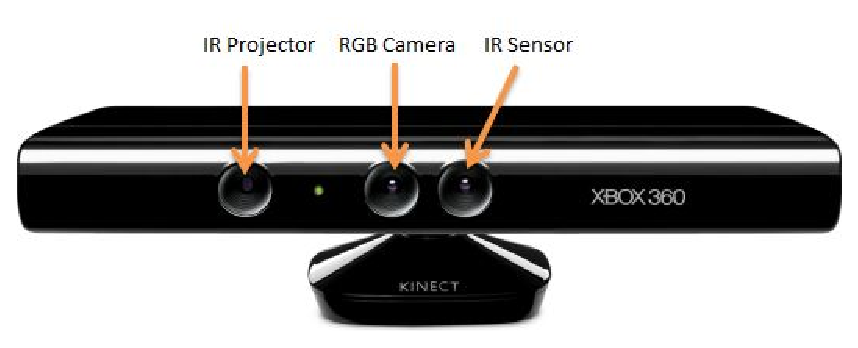
\includegraphics[scale=0.5]{img/kinect/kinect2.eps}
		% 	\caption[Kinect Sensors]{Kinect sensors: depth sensor and VGA camera location.}
		% 	\end{center}
		% \end{figure}


		The parts that compose the Kinect sensor are the following: 

		\begin{itemize}
			\item{\textbf{VGA camera}}\\
			The camera contained by the kinect has a pixel resolution of 640x480 and a frame rate of 30 fps. It is used mainly to provide the output data with the RGB components for each point. 
			
			\item{\textbf{Depth sensor}\\
			The depth sensor consists on an infra-red projector combined with a monochrome CMOS sensor. This latter measures the time it takes the light to come back after being reflected on the objects. Knowing the speed of light it can be easily obtained the distance of the objects from the depth sensor. 

			\item{\textbf{Multi-array microphone}}\\
			This array of four microphones are included because the kinect was designed as a gaming device. They are not used for the three-dimensional world retrieving. 

		\end{itemize}


\newpage
\newpage
\section{Object learning and recognition}

Object learning and recognition is an active field. 
In this section the most important works related to that field are presented. 
Also, the differences and improvements performed in this thesis with respect to the previous art are stated. 
% In this section the most important works related to this thesis are exposed. 

\subsection{Object learning and recognition using 2D and 3D input data}

This special branch in the object learning and recognition field has been active for many years. 
One of the first works in the field was the one performed by D.M.Gavrila and F.C.A. Groen. 
In 1992,  they developed a  system that performs 3D object recognition using 2D input data \cite{D.M.Gavrila1991}.
A 3D model was created and then the new 2D projection was matched to this model.
A geometric hashing method of matching was applied to the input 2D projection. 
The image was only matched to a model if the error to a nearby 2D projection was within certain thresholds.
The testing was performed under a controlled environment and using textured objects. 
The system would not give the same results in a real environment with noise and loosely defined objects. 
Also, the use of hashing limits the size of the dataset due to its high computing cost. 
\\

Later systems as \cite{Sheta2012} explore different descriptors for the objects that result less time-consuming. 
In this case, fuzzy logic is used to match the learned features to the new ones. 
Those descriptors are a set that include Affine \cite{Reiss:1991:RFT:117668.117680}, Zemike \cite{Teague} and Hu \cite{Hu1962} moments invariants among others. 
The results obtained a high percentage of true positives. 
But, again, the system uses a controlled setup:
The input is collected from three cameras that has a known illumination and orientation. 
The objects are white with significantly different shapes and they rest in a black background during learning and recognition phases. 
The applications in which it could be used are more related to the industrial field than the robotics field. 
\\

An outdoor system is described in \cite{Zia2013}, which demonstrated the effectiveness of two methods when combined: local descriptors and 3D wireframes. 
The system was able to distinguish between cars and bicycles and to estimate their pose. 
The input of the recognition is a single 2D image. 
Nevertheless, the training was made off-line, using a high number of Computer-Aided Design (CAD) model's views. 
\\

These systems differ with the one presented in this thesis in one major aspect: 
the user-software interaction. 
This thesis is based on providing an easy and intuitive interface. 
The learning process is performed easily and on-line and the recognition is real-time. 
There is no setting needed, no previous processing and care about the environment. 
The combination of 2D and 3D information in my system is, to the best of my knowledge, unique. 
The fact of recognizing the objects using those two different methods and then apply a decision algorithm better the results, reducing the effect of the noise.  



\subsection{In-hand object learning and recognition}

Most of the literature in object learning and recognition has been developed using wearable cameras as the input of the system. 
One of the most representative works is \cite{Roth2006}, which consists in a camera used to capture daily objects to construct a dataset more easily. 
Its main feature is that it eliminates the necessity of manually segmenting and labeling the learning datasets for object recognition libraries. 
It only learns new templates that are later fed to a off-line learning algorithm. 
\\

Another example is \cite{Philipose2009}, in which a benchmarking of an egocentric object recognition system is performed. 
This in-hand object recognition uses as input an image that has the object used at the center. 
The background is not segmented in this system because the errors produced by it may be neglected.
The object occupies most of the camera's frame and hence the processing of the input data to the system does not need to be as exhaustive as the one developed in this thesis.  
\\

The system presented here has a different approach: an in-hand object recognition and learning in which the user is located in front of the acquisition device. 
It is a solution to the same problem, the recognition of an object that a user holds, but the initial setting is different. 
In my thesis, the user is in front of the camera, because the software is running on a robot. 
The interaction between the software and the user is different from the previous art on the field. 
This change in the input creates an additional difficulty due to the hand's segmentation in the input image. 
\\

Furthermore, to the best of my knowledge there is no previous art in in-hand object learning and recognition using 2D and 3D information combined together. 
All of the algorithms described in this section use a camera and hence 2D data as input. 
The inclusion of 3D and the independence between the 2D and 3D recognition processes improve the noise resistance of my system with respect to the previous art. 


% \paragraph{Template matching}


% In the object recognition field obtaining good descriptors is of paramount importance. 
% The quality of the features extracted as the model of the object determine the quality of the algorithm. 
% Due to this importance, the next chapter is devoted to the descriptors that can be obtained from 2D and 3D data.




%%%%%%%%%%%%%%%%%%%%%%%%%%%%% 				DESCRIPTORS 				%%%%%%%%%%%%%%%%%%%%%%%%%%%%%%%%%%%%%%%%%%55


\section{Feature Extraction algorithms}
In chapter \ref{fundamentals} a brief introduction to the characteristics of the different feature extractor algorithms was performed. 
In this section the different state-of-the-art algorithms for 2D and 3D feature extraction are presented and compared. 

\subsection{Algorithms for 2D Feature Extraction}
\label{2d_features}


The most used algorithms for general object recognition are presented in this section. 
% due to their relation between performance, invariantness and speed are exposed below. 
They appear in chronological order and the differences, similarities and improvements between them are explained. 
The selection of one algorithm or another depends on the application.


\paragraph{SIFT}\mbox{}\\
\label{sift}

SIFT (Scale Invariant Feature Transform) is a scale and rotation invariant feature descriptor \cite{sift}. 
There are various papers in which the performance of SIFT is compared with other descriptors and one of the most representative is \cite{Mikolajczyk2005}. In it, it can be seen that SIFT 
outperforms the previous algorithms, mainly due to its combination of local information and relative strengths and orientations of gradients. This combination makes it more robust to illumination and viewpoint changes and to noise. 
\\

The SIFT algorithm is based on four main phases: 
The first step is to detect the scale-space extrema, i.e. the location of potential interest points that are invariant to scale and rotation. 
The next step is to test those potential keypoints and select the more relevant based on measures of their stability. 
Then, one or more orientations are assigned to each of the previously obtained keypoints based on local image gradient directions. 
The following operations are performed on data that has been transformed relative to the location, scale and orientation of these features. 
This grants the invariantness to these transformations. 
The final phase consists on the description of the selected keypoint transforming the local image gradients into a representation that is descriptive enough to permit the information of various levels of shape distortion and illumination change. 
\\

In order to minimize the cost of extracting such a distinctive features, a cascade filtering approach is used in order to apply the most time-consuming operations only at locations that pass an initial test. 
It can be used for on-line applications but it still has a latency that was later improved. 
In order to reduce that lag, there were different approaches previous to the apparition of algorithms such as ORB, that reduced it drastically \cite{orb}. 
As an example, in \cite{sift_fpga} the SIFT algorithm was implemented on a FPGA (Field Programmable Gate Array), improving its speed by an order of magnitude and thus allowing it to run in real-time.
\\

The main reason of the high computing time of SIFT features is the descriptor vector size. 
In the aim of creating a highly distinctive descriptor, the vector is over-dimensioned slowing the detection, description and matching processes. 
This over-dimension is patent in the duplication of information that could be removed without affecting in a high degree its descriptiveness. 
% In relation with object recognition, this algorithm has a good performance in medium cluttered spaces. If the image is cluttered, there will appear a number of features of the background that do not have a match in the given database. Hence, it will give false positives and the match will have a lower probability. 




\paragraph{SURF}\mbox{}\\

SURF (Speeded Up Robust Features) is a scale and rotation invariant interest point or keypoint detector and descriptor \cite{surf}. 
It is a proprietary algorithm that simplifies the detection, extraction of the descriptors and matching steps thus obtaining them much faster than previous algorithms without losing repeatability, distinctiveness or robustness. 
\\

SURF algorithm is composed of three main steps: 
The first step of the algorithm is to identify the interest points such as corners, blobs or T-junctions, i.e. a junction were two lines meet forming a T. 
Therefore, this algorithm will be useful when evaluating a textured object.
The next step is to represent the neighbourhood of the interest points as a feature vector. 
The final step is to match the descriptor vectors between different images, in order to stablish a recognition of a pattern. Usually the matching is performed using as a reference the distance between the vectors. 
In this part, it can be perceived that the size of the descriptor vectors affects directly the performance of the algorithm. SURF aims to reduce that size without losing distinctiveness in the features. 
\\
\newpage
The SURF algorithm appeared after SIFT and hence it is interesting to see the similarities and differences between the two. 
In section \ref{descriptors} it was seen the good results obtained when combining the local information and relative data regarding gradients. This algorithm is based on similar characteristics: 
First, an orientation based on the information extracted from a circular region with the interest point as its center is obtained. Then, a square region aligned to that orientation is described and the descriptor is extracted from it.  
\\

The experiments in \cite{surf} show that the performance of these descriptors equals and in some cases improves the one of the SIFT descriptors. Also, the SURF descriptors are much faster computed and matched due to its smaller size. 


\paragraph{ORB}\mbox{}\\

ORB (Oriented FAST and Rotated BRIEF) is a fast rotation invariant, noise resistant binary descriptor based on BRIEF \cite{orb}.
ORB authors claim that it is two orders of magnitude faster than SIFT while matching its performance in many situations. 
Nevertheless, since ORB is not scale invariant, if the scale difference is noticeable the SURF algorithm will outperform ORB. 
\\

The features used in ORB build on the Features from Accelerated Segment Test (FAST) \cite{fast} keypoint detector and the Binary Robust Independent Elementary Features (BRIEF) \cite{brief} descriptor. Both of this previous algorithms offer a good performance and computing time relation. Since neither of them had the orientation taken into account, the main improvement made by the ORB developers is to include this feature in the algorithm. Also, the computation of oriented BRIEF features was improved and an analysis of variance and correlation for this features created. 
\\

FAST is mainly used to find keypoints in real-time systems that match visual features. The orientation operator included in this algorithm is the centroid operator described in \cite{orientation_corners}. This technique is not computationally demanding and also, unlike SIFT, it returns a single dominant result. 
\\

BRIEF uses simple binary tests whose performance is similar to SIFT with regard to robustness to lighting, blur and perspective distortion, but it is sensitive to in-plane rotation. In order to eliminate this drawback, the lowest computing costing solution is to steer BRIEF accordingly with the orientation of the keypoints. 
\\

In the different tests in \cite{orb} can be seen that the percentage of inliers obtained with ORB are higher and do not variate as much as those obtained by SIFT or SURF. 
ORB is then a good alternative for the latter if the application does not need a scale invariant descriptor. 
Finally, it is noticeable that this algorithm is Open Source.
Both SIFT and SURF are patent protected and the use for research is permitted, but for commercial uses the payment of a fee is needed. % is since the previous ones are proprietary. 
For all the above reasons, the ORB algorithm is the one being used in the system developed in this thesis. 


\subsection{Algorithms for 3D Feature Extraction}
\label{3d_features}


Applied to 3D data, a feature is a characteristic that describes a point inside the data. Features or descriptors can be compared to determine whether the point described is the same in two different inputs. They are used in object recognition and there are many different descriptors that can be used. Each of them has a certain speed in its computing and a reliability and robustness associated.
\\

Depending on the application in which they appear the developer must select the features depending on the specifications. 
As an example, two geometric point features are the underlying surface's estimated curvature and the normal at a specific query point. 
Both are local features and they characterize the point using the information provided by its neighbors. 
There are two types of features: local and global. 
Local features are less time-expensive but they are less robust. 
This means that two different objects may obtain very similar local features.
Global descriptors implement different techniques to generalize the information obtained for keypoints or important points in the mesh. 
They take more time to compute but are more robust than the previous ones. 
Since in our application the speed is key, local features are being used. 
\\

There exist a number of 3D local features that are computed using combinations of different geometric characteristics of the points. 
As an example, the 3D SIFT descriptor \cite{Scovanner2007} is obtained performing the 3D gradient and magnitude for each pixel, which is directly derived from its computation in 2D. 
It is rotation and scale invariant but is very time-consuming. 
The 3D descriptors being used in this thesis are the Point Feature Histogram (PFH) features. 

\subsubsection{Point Feature Histogram (PFH)}
\label{pfh}

The Point Feature Histogram \cite{Rusu2008} is a local 3D descriptor. 
It is fast to compute but its level of detail is limited. 
They are computed approximating the geometry of a point's k-neighborhood with a few values. 
This fact results in the possibility of obtaining a similar set of points in a very different object. 
\\

The PFH descriptors are invariant to rotation, position and point cloud density. 
They also perform well with noisy data. 
The features are created representing the mean curvature around the query point using a histogram of values. 
The normals' direction and magnitude of the points in the k-neighborhood of that point are studied. 
\\

The Fast Point Feature Histogram (FPFH) \cite{Rusu} descriptor is also a local descriptor based in the PFH. 
It is faster because it considers only the direct relations between the query point and its neighbors.
This fact makes them less robust than the previous descriptors. 
This is the reason why the Point Feature Histogram descriptors are the ones being used in this thesis instead of the Fast Point Feature Histogram descriptors. 

% \newpage
% \section{Hardware }
This section shows the hardware specifications with which the testing was performed. 

\subsection{Computer}

\subsection{RGB-D sensor}







%%% METHODS
%\addcontentsline{toc}{part}{Methods}
\part*{Methods}
In the present part, the hardware and software used in the project are explained, as well as the new software developed. 
The first chapter presents the different libraries and technologies that aided in the development of the thesis. 
In the second chapter, the code that has been developed in the project is explained.
Finally, the third chapter covers the hardware that is utilized.


%\addcontentsline{toc}{chapter}{Libraries and technologies}
\chapter{Libraries and technologies}
%%%%%%% explain why those technologies are being used !!!!
% technologies being used: 
%section or whatever

OpenCV\cite{opencv} (Open Source Computer Vision) is a library that implements real-time computer vision algorithms. 

It is cross-platform and it is released under a BSD\cite{BSD} license.

\begin{figure}[h]
	\begin{center}
    
\includegraphics[scale=1]{img/opencv/logo.eps}
	\caption[OpenCV Logo]{OpenCV Logo}
	\end{center}
\end{figure}

\input{methods/pcl}
"The Robot Operating System (ROS) is a set of software libraries and tools that help you build robot applications. From drivers to state-of-the-art algorithms, and with powerful developer tools, ROS has what you need for your next robotics project. And it's all open source."\cite{ros}

\begin{figure}[h]
	\begin{center}
    
\includegraphics[scale=0.3]{img/ros/groovy.eps}
	\caption[ROS Groovy Logo]{ROS Groovy Logo}
	\end{center}
\end{figure}
 % here include all the packages that will be used in the code
%doxygen?? 

%\addcontentsline{toc}{chapter}{The Code}
\chapter{The Code}
  % diagrams & previous explanation of the code
  % nodes
  % communication between nodes
  % 
  
%%%%%%%%%% explain the reasons of chosing each library and method etc. !!!

%\addcontentsline{toc}{chapter}{Hardware}
\chapter{Hardware}
The hardware needed for the software of this project to work is an RGB-D sensor compatible with the openni\_launch ROS package previously mentioned, and a computer running a Linux distro. 
The sensor being used for the experiments presented in the following chapter is the Kinect of the Xbox 360. The reason of chosing this specific sensor is that it is cheaper than the other
and also more accesible. The drawback with respect to other sensors such as the Asus Xtion PRO LIVE\cite{xtion} is that it needs a separate power plug to work, and also its size is bigger. 
\\

The characteristics of the Kinect used are the following: 
%%%% complete with the characteristics that are now in the state of the art section --> they do not belong there!!





%%% RESULTS
%\addcontentsline{toc}{part}{Results}
\chapter{Results}
\label{results}

\addcontentsline{toc}{chapter}{Introduction}
\chapter*{Introduction}

% Intro

This bachelor's thesis consists on a software that implements an in-hand object learning and recognition using 2D and 3D information. 
\\

The code was designed to be running inside a robot. Hence, everything is modularized and all processes are designed to run in parallel. 

The hardware needed for this project is an RGB-D sensor and a computer. 

\addcontentsline{toc}{section}{What does the software do?}
\section*{What does the software do?}
% What does it do?
The input of the software is the image and the point cloud provided by the RGB-D sensor. The output of the system is different depending on the mode we are working. If the user is making it learn a new object, the output is the percentage of learning completed. On the other hand, if the user is utilizing the recognizing mode, the output of the system is the identifier of the object, i.e. the number that represents which object in the dataset seems to be more similar to the one being shown to it currently. 

%%%%%%%%%%%%%%%%%%%%%%%%%%%%%%%%%%PICTURE

\addcontentsline{toc}{section}{How can it be used?}
\section*{How can it be used?}
% How it is used?
From the beginning, a easy and intuitive human-machine interface was a must. In order to achieve this, this simple state 
machine was designed:

%%%%%%%%%%%%%%%%%%%%%%%%%%%%%%%%%%%%%PICTURE

The software only allows one hand being used at a time. It will select the hand that is located highest. 

In order to switch between the learning and recognizing modes of the program, the distance between the hand and the body
is being used: 

If the hand is stretched out towards the RGB-D sensor, the software will start learning. If it is closer to the body, 
it will launch the recognizing mode, which is the default. 

\addcontentsline{toc}{section}{General characteristics of the software}
\section*{General characteristics of the software}
% How is the code coded?

The Robotic Operating System is being used in this project since it has numerous features that allow a more efficient and 
easier implementation of software that has the characteristics described above. More information about this operating 
system may be found in the section.
%%%%%%%%%%%%%%%%%%%%%%%%%%(!!!!SECTION).

The software developed in this thesis is a ROS package. The last release might be downloaded from the following link. 
%%%%%%%%%%%%%%%%%%%%%%%%%%%%%%%%LINK


\addcontentsline{toc}{section}{Thesis structure}
\section*{ Thesis structure}

\section{Computing performance evaluation}
This section presents the results of the computing performance experiment. 
First, in section \ref{results_nodes}, the CPU and RAM usage of each of the nodes of the system is presented. 
Afterwards, in section \ref{results_topics}, the bandwidth and the publishing rate of each of the nodes is shown. 
	% \begin{itemize}
		% \item{\textbf{Package and nodes benchmarking}}
		\subsection{Nodes' CPU and RAM usage}
		\label{results_nodes}
		\\

			As it was explained in chapter \ref{methods}, the CPU and RAM usage is measured in the different nodes that compose the software. 
			There is a high difference in the CPU and RAM usage between nodes.
			The nodes that only perform a transformation of the data such as the converter node have a lower CPU and RAM consumption.
			The nodes that process the input images and point clouds have much higher values. 
			Figure \ref{node} shows the results of the experiment. 
\\

			The nodes with a higher computing consumption are the ROI segmenters and the feature extractors both 2D and 3D. 
			Since the 3D data has a higher size, the both the CPU and RAM usage of the nodes using 3D information is much higher than those processing 2D data. 
			The learner recognizer node also has a higher consumption than the converter, event handler or system output nodes. 
			This is because these perform simple conversions and computations of integers and floating data. 
			On the other hand, the learner recognizer node implements the state machine of the software. 
			This means it has to deal with a higher amount of data than the previous nodes. 
	\\

			The total CPU usage is lower than the 23\%, and the RAM usage of the whole software is of less than the 5\%. 
			Since the processing unit has 4 physical cores with two threads per core, the system needs less than one core to operate in real time. %the CPU consumption is of less than one physical core. 
			The computer used has 8 GB of RAM. 
			Using that number, the total RAM usage of the system is of 0.4 GB. 
			Figure \ref{node} shows that the CPU and RAM consumption of the third-party packages is very high. 
			The total CPU and RAM usage including the third-party packages is almost the double of the total of the OCULAR nodes. 
			This means that it is needed a computer featuring less than two cores (at 2.4 GHz) and less than 1 GB of RAM to be able to run the whole system on real time. 

\newpage 

\begin{table}[H]
\centering
\begin{tabular} {l c r@{.}l c r@{.}l }%c r@{.}l }
\toprule
\addlinespace[3mm]
   \multicolumn{1}{c}{\begin{center}\textbf{NODES}\end{center}} &
   % \multicolumn{3}{c}{\begin{center}\textbf{CPU USAGE(0 - 800)}\end{center}} &
   \multicolumn{3}{c}{\begin{center}\textbf{CPU USAGE(\%)}\end{center}} &
   \multicolumn{3}{c}{\begin{center}\textbf{RAM USAGE(\%)}\end{center}} &\\
\addlinespace[-3mm]
\midrule
Converter && %1&60 && 
0&20 && 0&50 \\
ROI segmenter 2D && %6&70 && 
0&84 && 0&50\\
ROI segmenter 3D && %106&70 &&
 13&34 && 1&50\\
Feature extractor 2D && %19&50 && 
2&44 && 0&10\\
Feature extractor 3D && %37&90 &&
 4&74 && 0&50\\
Event handler && %1&30 && 
0&16 && 0&50 \\
Learner recognizer &&% 8&30 && 
1&04 && 0&80 \\
System output && %1&00 && 
0&13 && 0&30 \\
\midrule
\textbf{TOTAL OCULAR NODES: } && %\textbf{183}&\textbf{00} &&
\textbf{22}&\textbf{88} && \textbf{4}&\textbf{70} \\
\midrule
pi\_tracker node: skeleton\_tracker && 4&86 && 3&2\\
openni\_launch nodelet && 16&19 && 1&00\\
\midrule
\textbf{TOTAL WITH THIRD-PARTY PACKAGES:} && %\textbf{183}&\textbf{00} &&
\textbf{43}&\textbf{84} && \textbf{8}&\textbf{90} \\
\bottomrule
\end{tabular}
\caption[Nodes' CPU and RAM usage]{Nodes' CPU and RAM usage}
\label{node}

\end{table}



			% \begin{figure}[h]
			% 	\begin{center}
			%     \includegraphics[width=\linewidth]{img/tests/node.png}
			% 	\caption[Nodes benchmarking]{Nodes benchmarking}
			% 	\label{node}
			% 	\end{center}
			% \end{figure}

		% \item{\textbf{Topic benchmarking}}\\
		\subsection{Topic network usage}
		\label{results_topics}

			The following figures \ref{hz} and \ref{bw} show the publishing rate and bandwidth of the different topics. 
			In figure \ref{hz}, the difference in the average rate between topics can be appreciated. 
			The publishing rate varies significantly between topics. 
			The first column shows the average number of messages published in each topic. 
			% It can be seen that those topics with lower-sized messages experiment a higher average publishing rate. 
			This is due to the reduced processing time and hence delay between message publishes. 
			All topics but one have a more or less similar average publishing rate.
			The bottle neck of the process that establishes the publishing rate is the kinect. 
			Since the information provided by this sensor is the input to most of the nodes of the system, their publishing rate is similar to the one of the kinect, 30 frames per second.  
			\\

			The only topic that publishes at a lower rate than the others is the final object ID topic. 
			This node transmits the output of the system, as was previously explained in section \ref{system_description}.
			The node that publishes it is buffering the object ID topic messages. 
			This creates a delay and the node publishes approximately one message per second in the final object ID topic. 
			% This knowledge matches the average rate observed of 0.75 messages per second. 
			% It is also confirmed when looking at the next column, in which the minimum time between messages is presented. 
			% All the previous topics have a zero or almost zero seconds. 
			% But final object ID observes a minimum time of around one second. 
				% This is reflected on the standard deviation column. 
			% The values for both object ID and final object ID, which are dependent on the system's event, are much higher than the rest of the topics. 

			\\


			Also it is noticeable the minimum rate column. 
			Most of the topics have a minimum publishing rate of 0 seconds.
			The only one that is different is the final object ID topic. 
			Another singular fact can be found in the maximum column. 
			All topics but two have less than 1 second as maximum publishing rate. 
			Those two are again final object ID and the object ID topic. 
			The reasons behind this particular behaviour are discussed in chapter \ref{discussion}. 
			\\

			The maximum column shows that the time between messages increases with the complexity of the processing performed by the node that publishes in that topic. 
			As an example, the segmented and descriptors topics have similar time, around half a second. 
			It is remarkable the value of the maximum time obtained by the object ID topic, which is the highest of the column. 
			% It was previously seen that this topic publishes the instant value of the estimated recognized object. 
			% The time between messages depend on the previous data transformation required. 
			% But also the event that the software is undergoing (learning or recognizing) affects that time. 
			The node that publishes in the object ID topic is the Learner-Recognizer node described in section \ref{learner_recognizer}.
			This node only publishes a message when the system is recognizing the objects. 
			If the system is learning new objects, there is no message published. 
			This could be the cause of the high result in the maximum time between messages column. 
			% When the system is learning, no estimations of the object ID are performed and hence no messages are published. 
			% On the other hand, when the system is recognizing, the topic is filled at a rate of almost thirty messages per second. 
			

			% \begin{figure}[h]
			% 	\begin{center}
			%     \includegraphics[width=\linewidth]{img/tests/topic_hz.png}
			% 	\caption[Topic benchmarking - Publishing rate]{Topic benchmarking - Publishing rate}
			% 	\label{hz}
			% 	\end{center}
			% \end{figure}

			\newpage

\begin{table}[H]
\centering
\begin{tabular} {l r@{.}l r@{.}l r@{.}l  r@{.}l  }
\toprule
\addlinespace[3mm]
   \multicolumn{1}{c}{\begin{center}\textbf{TOPIC}\end{center}} &
   \multicolumn{2}{c}{\begin{center}\textbf{\hspace*{-0.7cm}AVERAGE [Hz]}\end{center}} &
   \multicolumn{2}{c}{\begin{center}\textbf{MIN [s]}\end{center}} &
   \multicolumn{2}{c}{\begin{center}\textbf{MAX [s]}\end{center}} &
   \multicolumn{2}{c}{\begin{center}\textbf{STD DEV [s]}\end{center}} &\\

\addlinespace[-3mm]
\midrule
 Hand location & 27&56	&	0&00	&	0&04	&  \hspace*{0.5cm}	0&01 \\
 Segmented  image &  26&70	&	0&00	&	0&50	&	0&04\\
 Segmented  image  with  keypoints & 25&91	& 	0&00	&	0&50	&	0&03 \\
 Segmented  coordinates  (px) & 11&56 	&	0&05	&	0&13	&	0&03\\
 Segmented  point  cloud & 18&18 	&	0&05	&	0&26	&	0&01\\
 Descriptors  2D & 25&98 	&	0&00	&	0&50	&	0&03\\
 Descriptors  3D & 15&29 	&	0&00	&	0&42	&	0&05\\
 Event & 27&72  	&		0&00	&	0&04	&	0&01\\
 Object ID & 26&40 		&	0&00	&	4&23	&	0&21\\
 Final  object  ID & 0&75 	&	1&02	&	1&63	&	0&19\\
\bottomrule
\end{tabular}
\caption[Topic network usage - Publishing rate]{Topic network usage - Publishing rate}
\label{hz}
\end{table}



			% Table \ref{bw} shows the bandwidth consumed. 
			% It can be seen a huge difference between topics. 
			% The data ranges from the bytes to megabytes. 
			% The nodes using a bandwidth of bytes are segmented coordinates and final object ID. 
			% They are closely followed by the hand location, descriptors 2D, event and object ID topics that are in the kilobytes range. 
			% Finally, the ones using a higher bandwidth are the segmented image with and without keypoints, the segmented point cloud and the descriptors 3D topics. 
			% % \begin{figure}[h]
			% 	\begin{center}
			%     \includegraphics[width=\linewidth]{img/tests/topic_bw.png}
			% 	\caption[Topic benchmarking - Bandwidth]{Topic benchmarking - Bandwidth}
			% 	\label{bw}
			% 	\end{center}
			% \end{figure}






\begin{table}[H]
\centering
\begin{tabular} {l  c c c  }
\toprule
\addlinespace[3mm]
   \multicolumn{1}{c}{\begin{center}\textbf{TOPIC}\end{center}} &
   \multicolumn{1}{c}{\begin{flushright}\textbf{AVERAGE [kB/s]}\end{flushright}} &
   \multicolumn{1}{c}{\begin{flushright}\textbf{MIN [kB]}\end{flushright}} &
   \multicolumn{1}{c}{\begin{flushright}\textbf{MAX [kB]}\end{flushright}} &\\

\addlinespace[-3mm]
\midrule

Hand location & 1.38 &  0.12 	& 0.12  \\
Segmented image & 1.79$\cdot10^{3}$		&	60	&	60
\\
Segmented image with keypoints & $1.64$	&	60	&	60
\\
Segmented coordinates (px) & 212& 57 & 58 \\
Segmented point cloud & $1.48\cdot10^{3}$ & 	0	&	830
\\
Descriptors 2D & 29.48	&	0.81 &	1.26 
\\
Descriptors 3D & $2.60\cdot10^{3}$	&	140	&	170
\\
Event & 1.06&	0.05 &	0.06 
\\
Object ID & 1.39	&		0.03 & 		0.03 
\\
Final object ID & 1.15$\cdot10^{3}$	&		2$\cdot10^{3}$	&	2$\cdot10^{3}$	
\\
\midrule

\textbf{TOTAL: } & \textbf{6.65}$\mathbf{\cdot 10^{3}}$ && \\
\bottomrule

\end{tabular}
\caption[Topic network usage - Bandwidth]{Topic network usage - Bandwidth}
\label{bw}

\end{table}


% The  bandwidth results presented in figure \ref{bw} show the different sizes the data used have. 
			Figure \ref{bw} show the bandwidth measured in each of the system's topics. 
			There is a huge different in the results for the different topics, the numbers range from the bytes to the megabytes. 
			Those topics using custom messages use a higher bandwidth than those using a standard message such as a number. 
			\\

			This fact can be illustrated with the final object ID topic, which publishes integer messages and uses an average bandwidth of approximately 1 B/s. 
			The segmented coordinates in pixels topic is the one that has the next lowest bandwidth and its messages are vectors that contain two integers. 
			Its average bandwidth is around 200B/s. 
			\\

			In the kilobytes range, the hand location, descriptors 2D, event and object ID are located. 
			All but descriptors 2D are filled with custom made messages. 
			The data consists in integers and floats mixed with strings. 
			% For more information about custom messages, please read the chapter \ref{system_description}.
			It might be noted that the descriptors 2D topic is an order of magnitude higher than the other ones. 
			This is due to the fact that its messages are images and hence have a higher size than the other ones. 
			\\

			Finally, the megabytes range houses the segmented image topics as well as the segmented point cloud and the descriptors 3D. 
			All are filled with heavy messages that store two-dimensional and three-dimensional data.

	\end{itemize}
\section{ Evaluation of the object recognition accuracy}
\label{results_accuracy_measurement}
This sections presents the results obtained in the object recognition accuracy experiment. 
It was previously explained that the different objects may be learned using one or more views per template. 
The accuracy is analyzed depending on the number of views learned. 
The experiment was repeated using one, five and ten views in order to evaluate the influence of the number of views in the accuracy of the system. %were used and the same experiment was performed for each of them. 
The data in the confusion matrices shown below is normalized to a zero to one range to make them comparable.
% This is due to the fact that the publishing rate of the topics varies with the amount of templates. 
% Hence, for an experiment that lasts the same amount of time a larger number of messages would appear when the algorithm has 1 view templates. 
The discussion of the results can be found in section \ref{discussion}.

\subsection{Template using 1 view}
% This experiment was performed adding to the dataset one view per object. 
In this experiment, the system was trained using one view per object. 
Figure \ref{1view_matrix} shows the confusion matrix obtained with the experiment. 
The diagonal of the matrix are the success rates obtained for the different objects. 
The success rate is defined as the number of true positives over the total number of estimations returned by the system. 
From table \ref{1view_matrix} it can be seen that software has around a 50\% of success rate in all objects.
% This success rate is the ratio of true positives obtained, i.e. the number of times the system outputted the object that was being shown to it.
The F1-score obtained per object as well as their precision and recall values may be found in figure \ref{1view_fscore}.

	% \begin{figure}[H]
	% 	\begin{center}
	%     \includegraphics[width=\linewidth]{img/tests/1view_matrix.png}
	% 	\caption[Confusion matrix - templates using 1 view]{Confusion matrix using a template that stores one view per object. The results are given in a 0 to 1 range. }
	% 	\label{1view_matrix}
	% 	\end{center}
	% \end{figure}

	% \begin{figure}[H]
	% 	\begin{center}
	% 	\includegraphics[width=0.55\linewidth]{img/tests/1view_fscore.png}
	% 	\caption[F1-score - templates using 1 view]{F1-score calculation using the precision and recall parameters. Results for templates using one view per object. }
	% 	\label{1view_fscore}
	% 	\end{center}
	% \end{figure}



		\begin{table}[H]
		\centering
		\begin{tabular} {l r@{.}l r@{.}l r@{.}l r@{.}l r@{.}l r@{.}l }
		\toprule
		\addlinespace[3mm]
		   \multicolumn{1}{c}{\begin{center}\textbf{Real} \mid \textbf{Predicted}\end{center}} &
		   \multicolumn{2}{c}{\begin{flushright}\textbf{ball}\end{flushright}} &
		   \multicolumn{2}{c}{\begin{flushright}\textbf{skull}\end{flushright}} &
		   \multicolumn{2}{c}{\begin{flushright}\textbf{cup}\end{flushright}} &
		   \multicolumn{2}{c}{\begin{flushright}\textbf{bottle}\end{flushright}} &
		   \multicolumn{2}{c}{\begin{flushright}\textbf{mobile}\end{flushright}} &
		   \multicolumn{2}{c}{\begin{flushright}\textbf{calculator}\end{flushright}} &\\

		\addlinespace[-3mm]

		\midrule
		\textbf{ball}		&	\textbf{0}&\textbf{55}	&	0&00	&	0&03	&	0&14	&	0&28	&	0&00	\\
		\textbf{skull}		&	0&03	&	\textbf{0}&\textbf{45}	&	0&28	&	0&24	&	0&00	&	0&00	\\
		\textbf{cup}		&	0&00	&	0&03	&	\textbf{0}&\textbf{52}	&	0&14	&	0&28	&	0&03	\\
		\textbf{bottle}		&	0&21	&	0&00	&	0&03	&	\textbf{0}&\textbf{59}	&	0&17	&	0&00	\\
		\textbf{mobile}		&	0&14	&	0&03	&	0&14	&	0&10	&	\textbf{0}&\textbf{55}	&	0&03	\\
		\textbf{calculator}	&	0&07	&	0&00	&	0&07	&	0&14	&	0&21	&	\textbf{0}&\textbf{52}	\\
		\bottomrule
		\end{tabular}
		\caption[Confusion matrix - templates using 1 view]{Confusion matrix using a template that stores one view per object. The results are given in a 0 to 1 range. }
		\label{1view_matrix}
		\end{table}
	The bottle is the object with a higher success rate. 
	Nevertheless, the system recognized this object a high number of times when all the other objects of the dataset were presented to it. 
	Hence, the precision in the bottle recognition is low, as can be seen in figure \ref{1view_fscore}.
	Also, its recall is low because different objects such as the ball or the mobile were detected when the bottle was being presented to the software.  
	\\

	The ball has a precision and recall of exactly the same value. 
	It is a low value because there were false positives when the ball was being used. 
	The system recognized the bottle and the mobile a large number of times. 
	Also, the output of the system showed a ball when the bottle and the mobile were shown with high rates. 
	It also appeared when the calculator and the skull were presented but a lower and almost negligible amount of times. 
	\\

	The skull presents a very good precision. 
	It is almost negligible the amount of times it was detected when other objects were being held in front of the system. 
	Nevertheless, the recall is worse since the cup and the bottle were outputted a high amount of times when the skull was being used. 
	It could be because all three objects have very similar 2D texture, leading to matchable 2D descriptors. 
	\\

	The cup has a success rate of 0.52. Its precision, recall and F1 score values are around that number as well. 
	This is due to the fact that the system outputted the mobile's and the bottle's identification number a high number of times when the cup was being used. 
	Also, the software detected the cup when all the other objects were being presented to it. 
	\\

	The mobile has even a lower precision than the cup and the results are comparable to the previous ones. 
	The system detected the ball, the cup and the bottle when the mobile was being used a noticeable amount of times.
	Apart from that, the software recognized the mobile when all the other objects but the skull were presented a very high amount of times. 
	\\

	The calculator is the object with the best precision and F1 score of the dataset. 
	It can be seen that it was detected when other objects were shown to the system a negligible amount of times. 
	Nevertheless, when the calculator was being used the system outputted the mobile, the bottle with a high ratio and the cup and the ball with a lower one.
	Since the calculator is a heavily 2D textured object, is possible that a descriptor is very similar to other obtained in the mobile or the object. 
	Also, the 3D shape of calculator, mobile and bottle is similar and could lead to 3D confusions.  


\begin{table}[H]
\centering
\begin{tabular} {l l r@{.}l r@{.}l l r@{.}l }
\toprule
\addlinespace[3mm]
   \multicolumn{1}{c}{\begin{center}\textbf{Object}\end{center}} &
   \multicolumn{3}{c}{\begin{flushright}\textbf{Precision}\end{flushright}} &
   \multicolumn{2}{c}{\begin{flushright}\textbf{Recall}\end{flushright}} &
   \multicolumn{3}{c}{\begin{flushright}\hspace*{0.2cm}\textbf{F1 score}\end{flushright}} &\\
\addlinespace[-3mm]
\midrule
ball		&&	0&55 	&	0&55	&&	0&55	\\
skull		&&	0&87	&	0&45	&&	0&59	\\
cup			&&	0&48	&	0&52	&&	0&50	\\
bottle		&&	0&44	&	0&59	&&	0&50	\\
mobile		&&	0&37	&	0&55	&&	0&44	\\
calculator	&&	0&88	&	0&52	&&	0&65	\\
\bottomrule
\end{tabular}
\caption[F1-score - templates using 1 view]{F1-score calculation using the precision and recall parameters. Results for templates using one view per object. }
\label{1view_fscore}

\end{table}




\subsection{Template using 5 views}
In this experiment, five views were learned per object. 
The confusion matrix may be seen in figure \ref{5views_matrix}. 
Figure \ref{5views_fscore} shows the F1-score obtained in this measurement, as well as the precision and recall per object. 
	% \begin{figure}[H]
	% 	\begin{center}
	%     \includegraphics[width=\linewidth]{img/tests/5views_matrix.png}
	% 	\caption[Confusion matrix - templates using 5 views]{Confusion matrix using a template that stores five views per object. The results are given in a 0 to 1 range. }
	% 	\label{5views_matrix}
	% 	\end{center}
	% \end{figure}

	% \begin{figure}[H]
	% 	\begin{center}
	% 	\includegraphics[width=0.55\linewidth]{img/tests/5views_fscore.png}
	% 	\caption[F1-score - templates using 5 views]{F1-score calculation using the precision and recall parameters. Results for templates using five views per object. }
	% 	\label{5views_fscore}
	% 	\end{center}
	% \end{figure}

\begin{table}[H]
\centering
\begin{tabular} {l r@{.}l r@{.}l r@{.}l r@{.}l r@{.}l r@{.}l }
\toprule
\addlinespace[3mm]
   \multicolumn{1}{c}{\begin{center}\textbf{Real} \mid \textbf{Predicted}\end{center}} &
   \multicolumn{2}{c}{\begin{flushright}\textbf{ball}\end{flushright}} &
   \multicolumn{2}{c}{\begin{flushright}\textbf{skull}\end{flushright}} &
   \multicolumn{2}{c}{\begin{flushright}\textbf{cup}\end{flushright}} &
   \multicolumn{2}{c}{\begin{flushright}\textbf{bottle}\end{flushright}} &
   \multicolumn{2}{c}{\begin{flushright}\textbf{mobile}\end{flushright}} &
   \multicolumn{2}{c}{\begin{flushright}\textbf{calculator}\end{flushright}} &\\

\addlinespace[-3mm]

\midrule
\textbf{ball}		&	\textbf{0}&\textbf{83}	&	0&14	&	0&00	&	0&00	&	0&03	&	0&00	\\
\textbf{skull}		&	0&34	&	\textbf{0}&\textbf{62}	&	0&0	&	0&00	&	0&00	&	0&03	\\
\textbf{cup}		&	0&03	&	0&21	&	\textbf{0}&\textbf{66}	&	0&07	&	0&00	&	0&03	\\
\textbf{bottle}		&	0&14	&	0&14	&	0&00	&	\textbf{0}&\textbf{69}	&	0&00	&	0&03	\\
\textbf{mobile}		&	0&10	&	0&13	&	0&00	&	0&07	&	\textbf{0}&\textbf{67}	&	0&03	\\
\textbf{calculator}	&	0&10	&	0&21	&	0&00	&	0&07	&	0&00	&	\textbf{0}&\textbf{62}	\\


\bottomrule
\end{tabular}
\caption[Confusion matrix - templates using 5 views]{Confusion matrix using a template that stores five views per object. The results are given in a 0 to 1 range. }
\label{5views_matrix}
\end{table}

	% In figure \ref{5views_matrix} the confusion matrix of this experiment may be seen.
	% The figure \ref{5views_fscore} represents the F1 score computation per object.  
	The success rate represented in the diagonal of figure \ref{5views_matrix} is higher than the ones obtained in the previous experiment. 
	In this test, the object that obtained the highest success rate is the ball. 
	It can be observed that the system only recognized two different objects when the ball was presented to it: the skull and the mobile. 
	Nevertheless, the amount of times the software outputted the mobile can be neglected. 
	% The fraction of confusions because of the mobile are negligible. 
	\\

	The cup has a higher rate than the skull, a 0.66. 
	It is noticeable that the system outputted a cup only when it was shown to it. 
	This leads to the maximum precision possible, 1. %, which can be seen in figure \ref{5views_fscore}.
	Nevertheless, the system recognized the skull, the bottle and the ball and calculator when the cup was shown to it. 
	The two last objects were detected a negligible amount of times. \\

	The bottle has a ratio of 0.69. 
	Both the ball and the skull were outputted when the bottle was shown to the system. 
	The most probable reason is that all three objects have curved sides that could be almost identical in terms of PFH 3D descriptors. 
	Also, the calculator was recognized a negligible amount of times. 
	The bottle was detected when the cup, the mobile and the calculator were presented to the system. 
	Nevertheless, the ratio for all three of them is low, a 0.07. 
	\\

	The mobile has a success of 67\%. 
	It is remarkable that the precision obtained is very high, a 95 \%. 
	This is due to the fact that the mobile was only detected wrongly when the ball was being used in the experiment. 
	The recall of the system with this object is much lower, around the 70\%, due to the false positives returned by the software. 
	The system outputted the ball, the skull, the bottle and the calculator when the mobile was being presented to it. . 
	% It is remarkable that it was detected wrongly when the ball was shown. 
	% And in this case, the amount of false recognitions is low, a 0.3. 
	\\

	Finally, the calculator has a score of 0.62. 
	It was recognized in all previous measurements except when the ball was shown to the system. 
	Nonetheless, the ratio of false positives is negligible ( a 3\%). 
	The objects that were detected when the calculator was presented are the skull, the ball and the bottle. 
	Since the calculator has a very cluttered 2D texture it is possible that some descriptors are similar to the ones extracted in other objects. 
	\\

	Figure \ref{5views_fscore} shows that the object with a higher F1 score is the cup, thanks mainly to its extremely high precision.  
	All testing objects obtained similar scores, around the 70 \% except the skull and the ball. 
	This is because the high 3D similarity between both. 

\begin{table}[H]
\centering
\begin{tabular} {l l r@{.}l r@{.}l l r@{.}l }
\toprule
\addlinespace[3mm]
   \multicolumn{1}{c}{\begin{center}\textbf{Object}\end{center}} &
   \multicolumn{3}{c}{\begin{flushright}\textbf{Precision}\end{flushright}} &
   \multicolumn{2}{c}{\begin{flushright}\textbf{Recall}\end{flushright}} &
   \multicolumn{3}{c}{\begin{flushright}\hspace*{0.2cm}\textbf{F1 score}\end{flushright}} &\\
\addlinespace[-3mm]

\midrule
ball		&&	0&53 	&	0&83	&&	0&65	\\
skull		&&	0&43	&	0&62	&&	0&51	\\
cup			&&	1&00	&	0&66	&&	0&79	\\
bottle		&&	0&77	&	0&69	&&	0&73	\\
mobile		&&	0&95	&	0&67	&&	0&78	\\
calculator	&&	0&82	&	0&62	&&	0&71	\\


\bottomrule
\end{tabular}
\caption[F1-score - templates using 5 views]{F1-score calculation using the precision and recall parameters. Results for templates using five views per object. }
\label{5views_fscore}
\end{table}




\subsection{Template using 10 views}
The last experiment was performed introducing ten views per object in the dataset. 
Figure \ref{10views_matrix} represents the confusion matrix obtained. 
The F1-score and the precision and recall per object may be found in figure \ref{10views_fscore}.
	% \begin{figure}[H]
	% 	\begin{center}
	%     \includegraphics[width=\linewidth]{img/tests/10views_matrix.png}
	% 	\caption[Confusion matrix - templates using 10 views]{Confusion matrix using a template that stores ten views per object. The results are given in a 0 to 1 range. }
	% 	\label{10views_matrix}
	% 	\end{center}
	% \end{figure}

	% \begin{figure}[H]
	% 	\begin{center}
	% 	\includegraphics[width=0.55\linewidth]{img/tests/10views_fscore.png}
	% 	\caption[F1-score - templates using 10 views]{F1-score calculation using the precision and recall parameters. Results for templates using ten views per object. }
	% 	\label{10views_fscore}
	% 	\end{center}
	% \end{figure}

\begin{table}[H]
\centering
\begin{tabular} {l r@{.}l r@{.}l r@{.}l r@{.}l r@{.}l r@{.}l }
\toprule
\addlinespace[3mm]
   \multicolumn{1}{c}{\begin{center}\textbf{Real} \mid \textbf{Predicted}\end{center}} &
   \multicolumn{2}{c}{\begin{flushright}\textbf{ball}\end{flushright}} &
   \multicolumn{2}{c}{\begin{flushright}\textbf{skull}\end{flushright}} &
   \multicolumn{2}{c}{\begin{flushright}\textbf{cup}\end{flushright}} &
   \multicolumn{2}{c}{\begin{flushright}\textbf{bottle}\end{flushright}} &
   \multicolumn{2}{c}{\begin{flushright}\textbf{mobile}\end{flushright}} &
   \multicolumn{2}{c}{\begin{flushright}\textbf{calculator}\end{flushright}} &\\

\addlinespace[-3mm]

\midrule
\textbf{ball}		&	\textbf{0}&\textbf{93}	&	0&00	&	0&07	&	0&00	&	0&00	&	0&00	\\
\textbf{skull}		&	0&31	&	\textbf{0}&\textbf{69}	&	0&00	&	0&00	&	0&00	&	0&00	\\
\textbf{cup}		&	0&03	&	0&14	&	\textbf{0}&\textbf{76}	&	0&00	&	0&03	&	0&03	\\
\textbf{bottle}		&	0&03	&	0&14	&	0&00	&	\textbf{0}&\textbf{83}	&	0&00	&	0&00	\\
\textbf{mobile}		&	0&07	&	0&03	&	0&14	&	0&00	&	\textbf{0}&\textbf{72}	&	0&03	\\
\textbf{calculator}	&	0&21	&	0&00	&	0&00	&	0&03	&	0&00	&	\textbf{0}&\textbf{76}	\\


\bottomrule
\end{tabular}
\caption[Confusion matrix - templates using 10 views]{Confusion matrix using a template that stores ten views per object. The results are given in a 0 to 1 range. }
\label{10views_matrix}
\end{table}




	The ball is the object with the highest success rate, a 93\%. 
	This time it was only confused with the cup a 7\%. 
	When the skull, the calculator and the mobile were presented to the system, the ball was detected a 0.31, 0.21 and 0.07. 
	Also, the ball was recognized a negligible ratio when the cup and the bottle were shown. 
	These results are expressed as well in table \ref{10views_fscore}, the precision is much lower than the recall and the final F1 score is around a 70\%. 
	% Those results are high and may be attributed to the improvable segmentation performed in the system. 
	% Possible upgrades are explained in chapter \ref{conclusions}.
	\\
	
	The skull was detected correctly a 69\% of times, it was only confused with the ball. %due to their shape similarity already mentioned.
	The skull was also recognized when the cup, the bottle and the mobile were being used. 
	\\

	The cup had a success rate of 76\%. 
	The system recognized wrongly the skull 14 \% and the ball, the mobile and calculator a negligible amount of times. 
	The skull has a similar 2D texture, a white background with highly defined drawings on it. 
	This could be the reason of the system's error. 
	The cup was also detected when the ball and the mobile were shown to the system. 
	\\

	The bottle obtained a 89\% success rate. 
	The system only made a false recognition of the bottle when the calculator was being shown to it, and the ratio is negligigle. 
	The bottle was confused with the skull and the ball, for the sames reasons as the cup. 
	Those objects, the skull, the cup and the bottle have similar 2D features that may be matched wrongly. 
	\\

	The mobile obtained a 0.72 rate. 
	The cup, ball, skull and calculator were recognized badly. 
	The mobile was wrongly recognized only when the cup was being shown to the system and the ratio is negligible (0.3). 
	\\

	Finally, the calculator has a 76\% success rate. 
	The system detected the ball a 21\% of times in this measurement. 
	It is possible that the dense 2D textures of both the ball and the calculator affected the system in the matching process. 
	The calculator was recognized a negligible amount of times when the mobile and the cup were being used. 

\begin{table}[H]
\centering
\begin{tabular} {l l r@{.}l r@{.}l l r@{.}l }
\toprule
\addlinespace[3mm]
   \multicolumn{1}{c}{\begin{center}\textbf{Object}\end{center}} &
   \multicolumn{3}{c}{\begin{flushright}\textbf{Precision}\end{flushright}} &
   \multicolumn{2}{c}{\begin{flushright}\textbf{Recall}\end{flushright}} &
   \multicolumn{3}{c}{\begin{flushright}\hspace*{0.2cm}\textbf{F1 score}\end{flushright}} &\\
\addlinespace[-3mm]

\midrule
ball		&&	0&59 	&	0&93	&&	0&72	\\
skull		&&	0&69	&	0&69	&&	0&69	\\
cup			&&	0&79	&	0&76	&&	0&77	\\
bottle		&&	0&96	&	0&83	&&	0&89	\\
mobile		&&	0&95	&	0&72	&&	0&82	\\
calculator	&&	0&92	&	0&76	&&	0&83	\\

\bottomrule
\end{tabular}
\caption[F1-score - templates using 5 views]{F1-score calculation using the precision and recall parameters. Results for templates using five views per object. }
\label{10views_fscore}
\end{table}



	\subsection{Comparison of the experiments results using different number of views}

	In this subsection the results obtained in the three object recognition accuracy experiments are summarized and presented together. 
	This is performed to offer a more global view of the system's performance as a function of the number of templates being used. 
	Figures \ref{comparison_success} and \ref{comparison_fscore} present a compilation of all the data extracted from the experiments. 
	\\



	\begin{figure}[H]
		\begin{center}
	    \includegraphics[width=0.8\linewidth]{img/tests/comparison_success.png}
		\caption[Comparison of the success rate]{Comparison of the success rate when using templates with 1, 5 and 10 views per object.}
		\label{comparison_success}
		\end{center}
	\end{figure}

	\begin{figure}[H]
		\begin{center}
	    \includegraphics[width=0.8\linewidth]{img/tests/comparison_fscore.png}
		\caption[Comparison of the F1 score]{Comparison of the F1 score when using templates with 1, 5 and 10 views per object.}
		\label{comparison_fscore}
		\end{center}
	\end{figure}

	% % Figure \ref{comparison_success} presents the success rate obtained in each of the three experiments for each object. 
	% It can be extracted a correlation between the number of views being learned per object and the success rate of the system. 
	% The graph in figure \ref{comparison_success} shows that the higher the number of views is, the better the success rate is as well. 
	% Figure \ref{comparison_fscore} plots the F1 score obtained for each object in every of the experiments being performed on the system. 
	% The relation between the number of views and the F1 score is not as clear as the previous case. 
	% Most of the times, the F1 score ratio increases with the number of views. 
	% Nevertheless, in the case of the skull and the cup this statement is not fulfilled. 
	% A discussion of these comparisons may be found in section \ref{discussion}.

		In \ref{comparison_success} it can be seen that through the experiments the success rate for the different objects has increased. 
	The differences in this rate between objects are almost identical from one experiment to the other. 
	This demonstrates that the errors of the system due to 2D or 3D similarity between objects may be improved using a higher number of views. 
	On the other hand, figure \ref{comparison_fscore} shows that the improvement of the F1 score with the number of views is not as clear as it was in the case of the success rate. 
	It is particular the case of the skull. 
	When the views were increased from one to five, the system outputted the skull more when other objects were being used. 
	This reduced the skull's precision and even though the recall was improved, the final F1 score was affected and resulted lower than the experiment using 1 view.  
	The same phenomena occurred with the cup but when the number of views was increased from five to ten. 
	All the other objects increased their F1 score with the augment of the number of views. 
	% With lower number of views, the F1 score is lower than with higher amount of views. 





%%% DISCUSSION
%\addcontentsline{toc}{part}{Discussion}
\chapter{Evaluation of the system: Discussion}
\label{discussion}

This chapter covers the discussion of the tests results presented in the previous section, number \ref{results}.
It follows the same structure than the last two parts. 
First, the benchmarking of both the nodes and the topics is discussed. 
Afterwards, the results obtained in the accuracy experiment are explained and justified. 
%\\
Chapter \ref{conclusions} is devoted to the improvement of the system based on the observations performed on the experiments. 

\section{Computing performance evaluation}
	\subsection{Nodes' CPU and RAM usage}
		\\

			The nodes with a higher computing consumption are the ROI segmenters and the feature extractors both 2D and 3D. 
			Since the 3D data has a higher size, the usage of the nodes using 3D information is much higher than those processing 2D data. 
			\\
			The learner recognizer node also has a higher consumption than the converter, event handler or system output nodes. 
			This is because the last ones perform simple conversions and computations of integers and floating data. 
			On the other hand, the learner recognizer node implements the state machine of the software. 
			This means it has to deal with a higher amount of data than the previous nodes. 




		\paragraph{Topic benchmarking}\mbox{}\\

			Chapter \ref{results} presented the results of the topic benchmarking. 
			Two different characteristics were measured: the publishing rate and the bandwidth used. 
			That data can be found in the figures \ref{hz} and \ref{bw} respectively. 
			\\

			\begin{itemize}
				\item{\textbf{Publishing rate}}\\

			The publishing rate varies significantly between topics. 
			The first column shows the average number of messages published in each topic. 
			It can be seen that those topics with lower-sized messages experiment a higher average publishing rate. 
			This is due to the reduced processing time and hence delay between message publishes. 
			All topics but one have a more or less similar average publishing rate. 
			\\

			The one different topic is the final object ID. 
			This node transmits the output of the system, as was previously explained in chapter \ref{system_description}.
			The node that publishes it is buffering the object ID topic messages. 
			This creates a delay and the node publishes approximately one message per second in the final object ID topic. 
			This knowledge matches the average rate observed of 0.75 messages per second. 
			It is also confirmed when looking at the next column, in which the minimum time between messages is presented. 
			All the previous topics have a zero or almost zero seconds. 
			But final object ID observes a minimum time of around one second. 
			\\

			The maximum time shows results that increase with the complexity of the processing performed by the node that publishes in that topic. 
			As an example, the segmented and descriptors topics have similar time, around half a second. 
			It is remarkable the value obtained for the object ID topic. 
			It was previously seen that this topic publishes the instant value of the estimated recognized object. 
			The time between messages depend on the previous data transformation required. 
			But also the event that the software is undergoing (learning or recognizing) affects that time. 
			When the system is learning, no estimations of the object ID are performed and hence no messages are published. 
			On the other hand, when the system is recognizing, the topic is filled at a rate of almost thirty messages per second. 
			\\

			This is reflected on the standard deviation column. 
			The values for both object ID and final object ID, which are dependent on the system's event, are much higher than the rest of the topics. 

			\\

			\item{\textbf{Bandwidth}}\\

			The  bandwidth results presented in figure \ref{bw} show the different sizes the data used have. 
			The numbers range from the bytes to the megabytes. 
			The topics using custom messages use a higher bandwidth than those using a standard message such as a number. 
			\\

			This can be illustrated with the final object ID topic. 
			It publishes integer messages and its average bandwidth is around 1 B/s. 
			The next that follows in the lowest bandwidth is the segmented coordinates in pixels. 
			Its messages are vectors composed of two integers. 
			The average bandwidth is around 200B/s. 
			\\

			In the kilobytes range, the hand location, descriptors 2D, event and object ID are located. 
			All but descriptors 2D are filled with custom made messages. 
			The data consists in integers and floats mixed with strings. 
			For more information about custom messages, please read the chapter \ref{system_description}.
			It might be noted that the descriptors 2D topic is an order of magnitude higher than the other ones. 
			This is due to the fact that its messages are images and hence have a higher size than the other ones. 
			\\

			Finally, the megabytes range houses the segmented image topics as well as the segmented point cloud and the descriptors 3D. 
			All are filled with heavy messages that store two-dimensional and three-dimensional data. 
		\end{itemize}

\section{Evaluation of the object recognition accuracy}
	This section discusses the results obtained in the accuracy measurement experiment. 
	To consult them please refer to section \ref{results_accuracy_measurement}.
	Each different experiment is discussed in a different subsection.


	\subsection{Template using 1 view}
	Figure \ref{1view_matrix} shows the confusion matrix for the experiment. 
	The diagonal marked in blue color is the fraction of true positives obtained. 
	It can be seen that the software has around a 50\% of success in all objects. 
	Figure \ref{1view_fscore} presents the precision, recall and F1 score for each of the testing objects. 
	\\

	The bottle is the object with a higher success rate. 
	Nevertheless, the system recognized this object a high number of times when all the other objects of the dataset were presented to it. 
	Hence, the precision in the bottle recognition is low, as can be seen in figure \ref{1view_fscore}.
	Also, its recall is low because different objects such as the ball or the mobile were detected when the bottle was being presented to the software.  
	\\

	The ball has a precision and recall of exactly the same value. 
	It is a low value because there were false positives when the ball was being used. 
	The system recognized the bottle and the mobile a large number of times. 
	Also, the output of the system showed a ball when the bottle and the mobile were shown with high rates. 
	It also appeared when the calculator and the skull were presented but a lower and almost negligible amount of times. 
	\\

	The skull presents a very good precision. 
	It is almost negligible the amount of times it was detected when other objects were being held in front of the system. 
	Nevertheless, the recall is worse since the cup and the bottle were outputted a high amount of times when the skull was being used. 
	It could be because all three objects have very similar 2D texture, leading to matchable 2D descriptors. 
	\\

	The cup's results are similar to the ball's. 
	The precision and recall are similar in number and low. 
	The features extracted from this object were not descriptive enough.
	It was confused with the mobile and the bottle, probably due to the similarity in 2D texture as was the case with the skull. 
	Also, the cup was outputted when all the other objects in the dataset were being used, with a specially high ratio in the skull and mobile. 
	\\

	The mobile has even a lower precision than the cup and the results are comparable to the previous ones. 
	The system detected the ball, the cup and the bottle when the mobile was being used a noticeable amount of times.
	Apart from that, the software recognized the mobile when all the other objects but the skull were presented a very high amount of times. 
	\\

	The calculator is the object with the best precision and F1 score of the dataset. 
	It can be seen that it was detected when other objects were shown to the system a negligible amount of times. 
	Nevertheless, when the calculator was being used the system outputted the mobile, the bottle with a high ratio and the cup and the ball with a lower one.
	Since the calculator is a heavily 2D textured object, is possible that a descriptor is very similar to other obtained in the mobile or the object. 
	Also, the 3D shape of calculator, mobile and bottle is similar and could lead to 3D confusions.  


	\subsection{Template using 5 views}
	In figure \ref{5views_matrix} the confusion matrix of this experiment may be seen.
	The figure \ref{5views_fscore} represents the F1 score computation per object.  
	The success fraction represented in the diagonal of figure \ref{5views_matrix} has improved with respect to the previous experiment. 
	Now, the higher rated object is the ball. 
	It can be observed that the system only recognized two different objects when the ball was presented to it: the skull and the mobile. 
	The skull is similar to the ball in its 3D form, which could be the reason behind those false recognitions. 
	The fraction of confusions because of the mobile are negligible. 
	\\
	The skull has around a 0.6 success rate. 
	Most of the 40\% of recognitions were ball. 
	This supports the theory that the similarity between those objects can confuse the algorithms used for the recognition. 
	\\

	The cup has a higher rate than the skull, a 0.66. 
	It is noticeable that the system outputted a cup only when it was shown to it. 
	This leads to the maximum precision possible, 1, which can be seen in figure \ref{5views_fscore}.
	Nevertheless, the system recognized the skull, the bottle and the ball and calculator when the cup was shown to it. 
	The two last objects had a low rate and can be neglected. 
	The skull was recognized a ratio of 0.2, which is high. 
	The reason behind it could be the similarity in the 2D texture of skull and cup. 
	Both are white objects with drawings that contrast with that background. 
	\\

	The bottle has a ratio of 0.69. 
	Both the ball and the skull were outputted when the bottle was shown to the system. 
	The most probable reason is that all three objects have curved sides that could be almost identical in terms of PFH 3D descriptors. 
	Also, the calculator was recognized a negligible amount of times. 
	The bottle was detected when the cup, the mobile and the calculator were presented to the system. 
	Nevertheless, the ratio for all three of them is low, a 0.07. 
	\\

	The mobile has a success of 67\%. 
	It is remarkable that it was detected wrongly when the ball was shown. 
	And in this case, the amount of false recognitions is low, a 0.3. 
	Figure \ref{5views_matrix} shows that when the mobile was shown to the system, the skull, the ball and the bottle were detected. 
	The mobile has rounded corners and sides that could make 3D descriptors on those locations be similar to the previous objects. 
	Also, the mobile is white with details represented in the 2D texture. 
	This feature is common with the bottle and the cup. 
	For certain positions of the cup and the mobile the 2D projection could be similar and lead to obtain less representative descriptors of the object. 
	\\

	Finally, the calculator has a score of 0.62. 
	It was recognized in all previous measurements except when the ball was shown to the system. 
	Nonetheless, the ratio of false positives is negligible ( a 3\%). 
	The objects that were detected when the calculator was presented are the skull, the ball and the bottle. 
	Since the calculator has a very cluttered 2D texture it is possible that some descriptors are similar to the ones extracted in other objects. 
	\\

	Figure \ref{5views_fscore} shows that the object with a higher F1 score is the cup, thanks mainly to its extremely high precision.  
	All testing objects obtained similar scores, around the 70 \% except the skull and the ball. 
	This is because the high 3D similarity between both. 


	\subsection{Template using 10 views}
	The results of this experiment may be found in figures \ref{10views_matrix} and \ref{10views_fscore}. 
	It can be observed an improvement with respect to the previous measurements. 
	Now, all success rates of the objects are above the 69\%. 
	Also it can be seen that the number of false recognitions was reduced noticeably mainly in the bottle, mobile and calculator objects. 
	\\

	The ball is the object with highest success rate, a 93\%. 
	This time it was only confused with the cup a 7\%. 
	When the skull, the calculator and the mobile were presented to the system, the ball was detected a 0.31, 0.21 and 0.07. 
	Also, it was recognized a negligible ratio when the cup and the bottle were shown. 
	Those results are high and may be attributed to the improvable segmentation performed in the system. 
	Possible upgrades are explained in section \ref{conclusions}.
	\\
	
	The skull was detected correctly a 69\% of times. 
	It was only confused with the skull due to their shape similarity already mentioned.
	The skull was also recognized when the cup, the bottle and the mobile were being used. 
	\\
	The cup had a success rate of 76\%. 
	The system recognized wrongly the skull 14 \% and the ball, the mobile and calculator a negligible amount of times. 
	The skull has a similar 2D texture, a white background with highly defined drawings on it. 
	This could be the reason of the system's error. 
	The cup was also detected when the ball and the mobile were shown to the system. 
	\\

	The bottle obtained a 89\% success rate. 
	The system only made a false recognition of the bottle when the calculator was being shown to it, and the ratio is negligigle. 
	The bottle was confused with the skull and the ball, for the sames reasons as the cup. 
	Those objects, the skull, the cup and the bottle have similar 2D features that may be matched wrongly. 
	\\
	The mobile obtained a 0.72 rate. 
	The cup, ball, skull and calculator were recognized badly. 
	The mobile was wrongly recognized only when the cup was being shown to the system and the ratio is negligible (0.3). 
	\\
	Finally, the calculator has a 76\% success rate. 
	The system detected the ball a 21\% of times in this measurement. 
	It is possible that the dense 2D textures of both the ball and the calculator affected the system in the matching process. 
	The calculator was recognized a negligible amount of times when the mobile and the cup were being used. 
	\\

	Figure \ref{10views_fscore} presents much better results than the previous experiments (Figures \ref{1view_fscore} and \ref{5views_fscore}).
	The bottle is the object with a higher F1 score. 
	It is noticeable that the bad precision presented in the ball recognition limited its F1 score result. 


	\subsection{Comparison of the experiments results using different number of views}
	Figures \ref{comparison_success} and \ref{comparison_fscore} present a compilation of all the data extracted from the experiments. 
	In \ref{comparison_success} it can be seen that through the experiments the success rate has increased. 
	The differences between objects are almost identical from one experiment to the other. 
	This demonstrates that the errors of the system due to 2D or 3D similarity between objects may be improved using a higher number of views. 
	\\
	On the other hand, in \ref{comparison_fscore} it can be seen that the improvement with the number of views is not the same as the success rate. 
	It is particular the case of the skull. 
	When the views were increased from one to five, the system outputted the skull more when other objects were being used. 
	This reduced the ball's precision and even though the recall was improved, the final F1 score was affected.  
	The same phenomena occurred with the cup but when the number of views was increased from five to ten. 
	All the other objects obtained normal results. 
	With lower number of views, the F1 score is lower than with higher amount of views. 
	The results of the experiment using ten views are very promising. 
	Further measurements with higher amount of views could be performed to determine the optimum balance between F1 score and processing requirements. 


%%% CONCLUSIONS
%\addcontentsline{toc}{part}{Conclusions}
\chapter{Conclusions}
\label{conclusions}
%intro al revés:
%contributions primero 
%cómo han resuelto las soluciones el problema
%cambio del contexto (future work)


%partes finales del trabajo: conclusiones, bibliografia y anexos
\backmatter

% bibliography %
%%\addcontentsline{toc}{chapter}{Bibliography}
\bibliography{tfg}{}	%poner el archivo .bib
\bibliographystyle{plain}


\appendix
\begin{appendices}

	
\section {Appendix: Regulatory compliance}

% It must be noted that since the project is a research project, most of the regulations here exposed may not be needed. 
% Nevertheless, they must be taken into account in the case that the system is commercialized.

	% \paragraph{ISO}\mbox{}\\

	% The International Organization for Standardization is an international organism that settles international standards. 
	% It has several joint committees with the International Electrotechnical Commission (IEC). 
	% They develop standards in different technical fields such as the electrical, electronic or IT fields. 
	% \\

	% The Information Technology (IT) term is related to the use of computers and telecommunications to interchange, store and manipulate data.  
	% It is a broad field in which the present project may be included.
	% The Joint Technical Committee devoted to this subject is the ISO/IEC JTC 1. 
	% Its main mission is develop, maintain, promote and facilitate IT standards regarding different areas such as the following : 
	% \begin{itemize}
	% 	\item{Design and development of systems and tools}
	% 	\item{Define performance and quality standards}
	% 	\item{Security, interoperability and portability of IT systems and products}
	% 	\item{Unified tools and environments as well as harmonized IT vocabulary}
	% \end{itemize}

	% This Committee has recently included the regulations regarding assistive tecnology (AT) \cite{japan1}\cite{japan2}.
	% %--> http://en.wikipedia.org/wiki/ISO/IEC_JTC_1 [IT projects] 


	% \paragraph{Software regulations}\mbox{}\\
		% This section is centered on the ones related to Open Source systems, since the software developed in this thesis is Open  
	The present section covers the regulatory compliance that affects directly to the system presented. 
	% There are different regulations regarding software. 
	% Since the project is Open Source, this section focus on presenting the regulations of this type of systems. \\
	Nowadays, the author of the software has the right of sharing it using a contract. 
	In it he determines which of the author rights he is going to yield and under what conditions. 
	This type of contract is called a software license. 
	% This project uses a number of third-party libraries that have their own license. 
	Sections \ref{ocular} to \ref{pcl} show the details of the licenses of this thesis and the third-party libraries being used. 

	\subsection{OpenCV}
	The Open Source Computer Vision library is released under a BSD license. 
	Hence it is free for both academic and commercial use. 
	Nevertheless, there are certain algorithms implemented whose license is different from the whole library. 
	The SIFT or SURF descriptors are two examples of this fact: they have a software patent. 
	This legal figure allows the use of the algorithms for investigation purposes, but imposes the payment of a fee for commercial uses. 
	Since OCULAR is intended to be an Open Source system, neither of these algorithms are used.
	Instead, the ORB algorithm is utilized in the system.% as the descriptor extractor of the system. 
	ORB has no patent and hence can be incorporated in software designed for both commercial and research uses. 

	\subsection{PCL}
	\label{pcl}
	The Point Cloud Library has as well a BSD license. 
	It is then free for commercial and research use. 
	Further information about the library and its license may be found in this \href{http://pointclouds.org}{\color{blue} {webpage}} \footnote{http://pointclouds.org}. 


	\subsection{ROS}
	All ROS core code is distributed under a BSD license, more specifically a BSD 3-Clause license. 
	It is very similar to the OCULAR license, the redistribution is permitted under certain conditions. 
	More information may be found in this \href{http://opensource.org/licenses/BSD-3-Clause}{\color{blue} {webpage}}\footnote{http://opensource.org/licenses/BSD-3-Clause}. 
	The different ROS packages that are used in this thesis (openni\_camera, openni\_launch and pi\_tracker) are distributed under a BSD license, according to their web pages ( \href{http://wiki.ros.org/openni_camera}{openni\_camera}\footnote{http://wiki.ros.org/openni_camera}, \href{http://wiki.ros.org/openni_launch}{openni\_launch}\footnote{http://wiki.ros.org/openni_launch}, \href{http://wiki.ros.org/pi_tracker}{pi\_tracker} \footnote{http://wiki.ros.org/pi\_tracker}).


	\subsection{OCULAR}
	\label{ocular}
	The license of this system must be coherent with the ones of the third-party libraries it uses.
	In fact, Open Source packages and libraries were selected to ensure that the whole system could be free for commercial and research use. 
	This is the reason why this project is being distributed with a MIT License (MIT). 
	The MIT license may be found in this  \href{https://raw.githubusercontent.com/irenesanznieto/ocular/master/LICENSE.md}{\color{blue}\underline {link}}\footnote{https://raw.githubusercontent.com/irenesanznieto/ocular/master/LICENSE.md}, and states the following: \\

	"Copyright (c) 2014 Irene Sanz Nieto

Permission is hereby granted, free of charge, to any person obtaining a copy of this software and associated documentation files (the "Software"), to deal in the Software without restriction, including without limitation the rights to use, copy, modify, merge, publish, distribute, sublicense, and/or sell copies of the Software, and to permit persons to whom the Software is furnished to do so, subject to the following conditions:

The above copyright notice and this permission notice shall be included in all copies or substantial portions of the Software.

The software is provided "as is", without warranty of any kind, express or implied, including but not limited to the warranties of merchantability, fitness for a particular purpose and noninfringement. In no event shall the authors or copyright holders be liable for any claim, damages or other liability, whether in an action of contract, tort or otherwise, arising from, out of or in connection with the software or the use or other dealings in the software."
\\

	The last paragraph is published in uppercase letters, but it was converted to lowercase to avoid a disturbance in the structure of the thesis. 	
	The license claims that software is available for redistribution and use, but no warranty is provided with it. 
	The different algorithms and third-party packages were selected taking into account that their licenses must be compatible with the one being provided by this system. 
	In the next sections the licenses under which the different packages are distributed are presented. 
	\\

	Apart from the licensing of the software, it was taken into account in the development of the system that this project needs to store the information learned to be able to use it in later sessions. % involves taking personal information to construct a dataset with which recognize different objects. 
	In order to observe the data protection Spanish law (Ley Orgánica 15/1999, de 13 de diciembre, de Protección de Datos de Carácter Personal), the stored data does not contain any personal information. 
	Instead of storing, for example, an image of the user, the information retrieved is a matrix of numbers containing the descriptors extracted from the objects. 
	This ensures that the system could be used in commercial software or that further investigations could be performed accordingly with the law. 





	% \paragraph{Data protection} \mbox{}
	\\

	% Since this project implements a proof of concept, the experiments performed with it were done by the author. 
	

	% This law "warrants and protects the personal data treatment, the public liberties and the fundamental rights of the persons, specially their honor and personal and familiar intimacy".
	% It is applicable to all data stored in a physical support. 
% 	Privacidad y confidencialidad: cualquier investigación que contenga datos de caracter personal tiene que cumplir los preceptos de la legislación de protección de datos. En España la norma que regula estos aspectos es la Ley Orgánica 15/1999, de 13 de diciembre, de Protección de Datos de Carácter Personal, cuayo objeto es 'garantizar y proteger en lo que concierne al tratamiento de los datos personales, las libertades públicas y los derechos fundamentales de las personas físicas, y especialmente de su honor e intimidad personal y familiar”.
% La ley es de aplicación a los datos de carácter personal registrados en cualquier soporte físico. El tratamiento de los datos cubre las actividades de recolección, registro, almacenamiento, recuperación, consulta, uso y diseminación. Para garantizar el derecho a la protección de datos, es necesario informar a las personas implicadas y solicitar su consentimiento para el tratamiento de sus datos. 

		\section{Appendix: Project management}
	\label{project_management}
		 The present section describes the project management followed in this thesis. The Gantt diagram created for this purpose can be seen in the following page.
		 \\

		 The thesis was started on February 7th 2013 and was finished on July 11th 2014.    
		 The project management has suffered modifications throughout its development.  The final project management chart has three differentiated parts the learning phase, the project programming and the documentation phase. 
\\

		 \begin{table}[H]
\centering
\begin{tabular} {l c c c }
\toprule
\addlinespace[3mm]
   \multicolumn{1}{c}{\begin{center}\textbf{PHASE}\end{center}} &
   \multicolumn{1}{c}{\begin{center}\textbf{BEGIN DATE}\end{center}} &
   \multicolumn{1}{c}{\begin{center}\textbf{END DATE}\end{center}} &
   \multicolumn{1}{c}{\begin{center}\textbf{\hspace*{0.7cm}DAYS}\end{center}} &\\
\addlinespace[-3mm]
\midrule
Planning of the Thesis 	&	07/02/13 	&	25/02/13	&	18 \\	
State of the art	&	28/04/13	&11/07/14	&	439	\\
Learning 		&	26/02/13	&	29/10/13	&	185	** \\
\hspace*{0.5cm}	OpenCV	&	26/02/13 	&	24/04/13 	&	57	\\
\hspace*{0.5cm}	OpenCV Demo	&	25/04/13	&	25/04/13	&	MILESTONE	\\
\hspace*{0.5cm}	PCL + ROS	&	25/04/13	&	29/10/13	&	127	**		\\
\hspace*{0.5cm}	PCL + ROS Demo	&	30/10/13	&	30/10/13	&	MILESTONE	\\
Project Objectives Definition	&	30/10/13	&	07/11/13	&	8\\	
Design	&	08/11/13	&	21/11/13 	&	13	\\
Project Programming		&	22/11/13	&	20/05/14	&	179	\\
\hspace*{0.5cm}	pi\_tracker integration : converter &	22/11/13	&	20/01/14	&	59\\	
\hspace*{0.5cm}	ROI segmentation implementation		&	21/01/14	&	20/02/14	&	30	\\
\hspace*{0.5cm}	Feature extraction implementation	&	21/02/14	&	15/04/14	&	53\\	
\hspace*{0.5cm}	State machine implementation	&	16/04/14	&	14/05/14	&	28	\\
\hspace*{0.5cm}	Decision algorithm development	&	15/05/14	&	20/05/14	&	5	\\
\hspace*{0.5cm}	Tests	&	22/11/13	&	20/05/14	&	179\\	
Documentation	&	21/05/14	&	11/07/14	&	51	\\
\hspace*{0.5cm}		Thesis writing	&	21/05/14	&	22/06/14	&	32	\\
\hspace*{0.5cm}		Thesis hand-in	&	22/06/14	&	22/06/14	&	MILESTONE	\\
\hspace*{0.5cm}		Presentation preparation		&	23/06/14	&	11/07/14	&	18	\\
\hspace*{0.5cm}		Thesis presentation		&	11/07/14	&	11/07/14	&	MILESTONE	\\

\addlinespace[3mm]
\bottomrule
\addlinespace[3mm]

\textbf{TOTAL DAYS: 	}		&&&\textbf{	454}	\\
\textbf{TOTAL HOURS (3h per day) :} &&&			\textbf{1362}	\\
\addlinespace[3mm]

\bottomrule
\end{tabular}
\caption[Days and hours per project phase]{Summary of the days and hours spent in each of the project's phases.\\
** 60 days of holidays are not taken into account in the calculations.}	

\label{phases}

\end{table}
\vspace*{0.5cm}


	Figure \ref{phases} presents a summary of the hours dedicated to each of the phases of the project. 
	These thesis parts are the following: 

		 \begin{itemize}
		 		\item{\textbf{Planning of the thesis}} \\
		 		In this phase a first research on computer vision and the different methods and algorithms used in object learning and recognition was performed. 
		 		The outline of the thesis planning based on the acquired knowledge was created. 

			 	\item{\textbf{State of the art}} \\
			 	This part is the most time-consuming.
			 	It consisted on the profound research and understanding of the different methodologies and algorithms devoted to computer vision in general and in-hand object recognition in particular. 
			 	Also, it includes the learning and understanding of third-party packages in order to use them later on in the project's development. 
			 	Figure \ref{gantt_diagram} shows that this phase was developed in parallel with the other ones. 
\newpage
			 	\item{\textbf{Learning phase}} \\
			 	This part consisted on a exploration of all the different technologies that could be used and the different state of the art techniques available. A thorough research on the object recognition and human tracking fields was performed. This research continued until the finishing of the thesis, but the most important part of it was made in this period of time. 
			 	The methods found were tested through demonstrations and there the main problems and possible solutions were obtained. This phase was crucial for the project, since in it the requisites of the software were defined as well as the technologies used and the general skeleton of the project's design that would later be implemented. 
			 	\\

			 	\item{\textbf{Project objectives definition}} \\
			 	After the learning and first learning of computer vision algorithms, the objectives of the project were defined. 
			 	They can be consulted in section \ref{objectives}. 

			 	\item{\textbf{Design}} \\
			 	This phase consisted on the design of the software that has been developed in this thesis. 
			 	In this part the project's requirements were created. 
			 	This document can be found in section \ref{requirements}. 
			 	The requirements document content was followed during the programming phase. 

			 	\item{\textbf{Project programming}}\\
			 	In this phase the project was coded and tested. The state of the art algorithms research continued to allow the overcoming of the different difficulties that appear when implementing theoretical concepts. This modified the project's design as well as some of the technologies applied in the thesis. 

			 	\item{\textbf{Documentation}}\\
			 	This final part of the project consisted on creating the documentation of the project and the present thesis. 
			 	Also, the presentation documentation was prepared. 
			 	\\
		 \end{itemize}

		 \newpage
		\begin{figure}[H]
			\centering
		    \includegraphics[scale=0.5, angle=90]{img/final.png}
			\caption[Gantt Diagram]{Gantt Diagram that specifies the different phases of the project and the time devoted to each of them. }	
			\label{gantt_diagram}
		\end{figure}


	\chapter{Appendix: \\Software requirements specification}
		\label{requirements}
		% % Author and supervisor
		\begin{minipage}{0.55\textwidth}
		\begin{flushleft} \large
		\emph{Author:}\\
		Irene Sanz Nieto\\
		\end{flushleft}
		\end{minipage}
		\begin{minipage}{0.4\textwidth}
		\begin{flushright} \large
		\emph{Supervisor:}\\
		Victor González Pacheco\end{flushright}\end{minipage}\vfill
			% \includepdf[pages={-}]{backmatter/requisites/requisites.pdf}
		\documentclass{article}
\usepackage[utf8]{inputenc}
\usepackage{amsmath}
\usepackage{graphicx}
\usepackage{listings}
\usepackage[top=1.55cm, bottom=2.29cm, left=1.6cm, right=1.47cm]{geometry}
% This is for the fancy title in each page
\usepackage{fancyhdr}
\lhead{}
\chead{}
\rhead{First Session: Combinational Design}
\pagestyle{fancy}

\usepackage{enumitem}


\makeatletter
\def\threedigits#1{\expandafter\@threedigits\csname c@#1\endcsname}
\def\@threedigits#1{%
  \ifnum#1<100 0\fi
  \ifnum#1<10 0\fi
  \number#1}
\makeatother
\AddEnumerateCounter{\threedigits}{\@threedigits}{100}


%\setenumerate[1]{}


\begin{document}

%%%% FRONTPAGE %%%%%%%%%%%%%%%%%%%%%%%%%%%%%%%%%%%%%%%%%%%%%%%%%%%%%%%%%%%
\begin{titlepage}

\begin{center}
%
\includegraphics[width=0.25\textwidth]{./uc3m.jpg}\\[2cm]
\textsc{\huge Bachelor's Thesis:\\[0.5cm]In-hand object detection and tracking using\\[0.5cm]2D and 3D
information }\\[4cm]


% Title
{\Huge\bfseries{Software Requirements Specification}\\[2cm]}

\Large{Version 0.2}
\\[11cm]


% Author and supervisor
\begin{minipage}{0.55\textwidth}
\begin{flushleft} \large
\emph{Author:}\\
Irene Sanz Nieto\\
\end{flushleft}
\end{minipage}
\begin{minipage}{0.4\textwidth}
\begin{flushright} \large
\emph{Supervisor:}\\
Victor González Pacheco\end{flushright}\end{minipage}\vfill

% Bottom of the page
{\large \today}

\end{center}
\end{titlepage}

%
\newpage
%
%%%%%%Table of contents%%%%%%%%%%%%%%%%%%%%%%%%%%%%%%
%%%%%%%%%%%%%%%%%%%%%%%%%%%%%%%%%%%%%%%%%%%%%%%%%%%%%
\tableofcontents
\newpage


%%%%%%Document%%%%%%%%%%%%%%%%%%%%%%%%%%%%%%%%%%
%%%%%%%%%%%%%%%%%%%%%%%%%%%%%%%%%%%%%%%%%%%%%%%%%%%%%
\section{Introduction}
\hspace{0.5cm}The project consists on an in-hand object learning and recognition software. 
%
\includegraphics[width=0.25\textwidth]{./uc3m.jpg}\\[2cm]
\subsection{Nodes}

\subsubsection{Event Handler Node}
	This node will identify the different user's gestures and act accordingly using a State Machine structure. 
	\begin{center}
		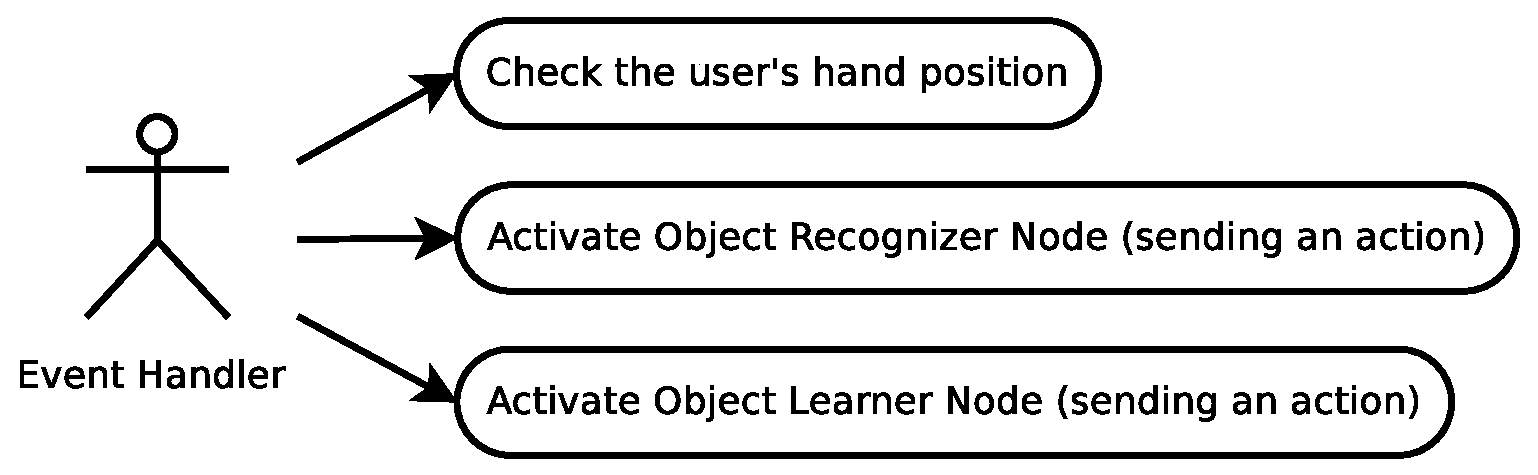
\includegraphics[scale=0.4]{../diagrams/images/uc_event_handler.eps}
	\end{center}
	
\subsubsection{Display Node}
This node shows the output of the program. There is a window in which different information will be shown. 
	\begin{center}
		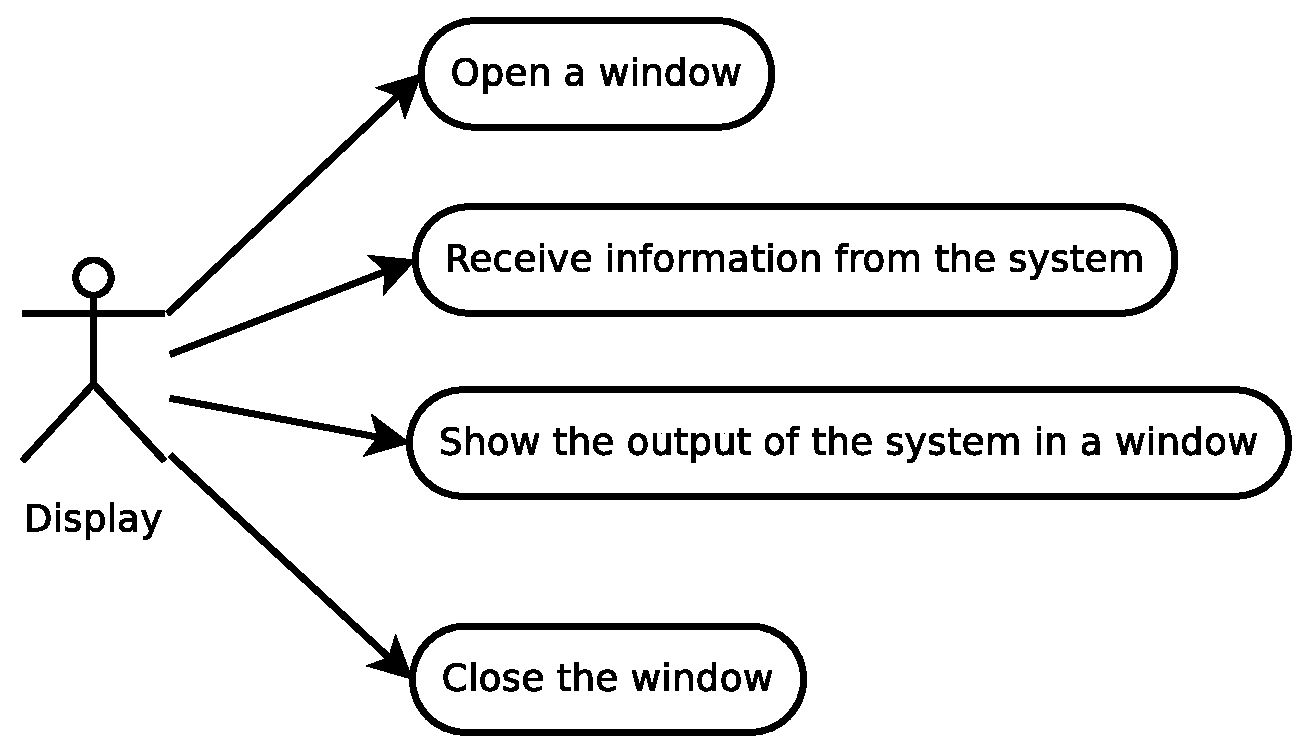
\includegraphics[scale=0.4]{../diagrams/images/uc_display.eps}
	\end{center}
	
\subsubsection{Object Learner Node}

\hspace{0.5cm}This node learns 2D and 3D features extracted from the handheld object using a RGB-D sensor.   

The sequence of the object learning is the following:
\\
First, 3D and 2D descriptors are extracted and written to a file. Then, two algorithms are trained (one for 2D and the other for the 3D template). The parameters of each trained algorithm are stored in a file. There will be hence one file per learned object and one file per algorithm.
\\

The learning of the objects is done in-hand. The training starts when the user extends the hand in front of the body, showing the new object to the RGB-D sensor. Then, the user rotates the object to allow the software to extract the features of different views to obtain a more robust model of the object. This way of learning new objects will allow a more intuitive interaction human-robot. When the user returns the arm to a position which is closer to the body, the algorithm starts learning the new object and after the learning, it comes back to the recognizing mode, which is the default. 

\begin{center}

		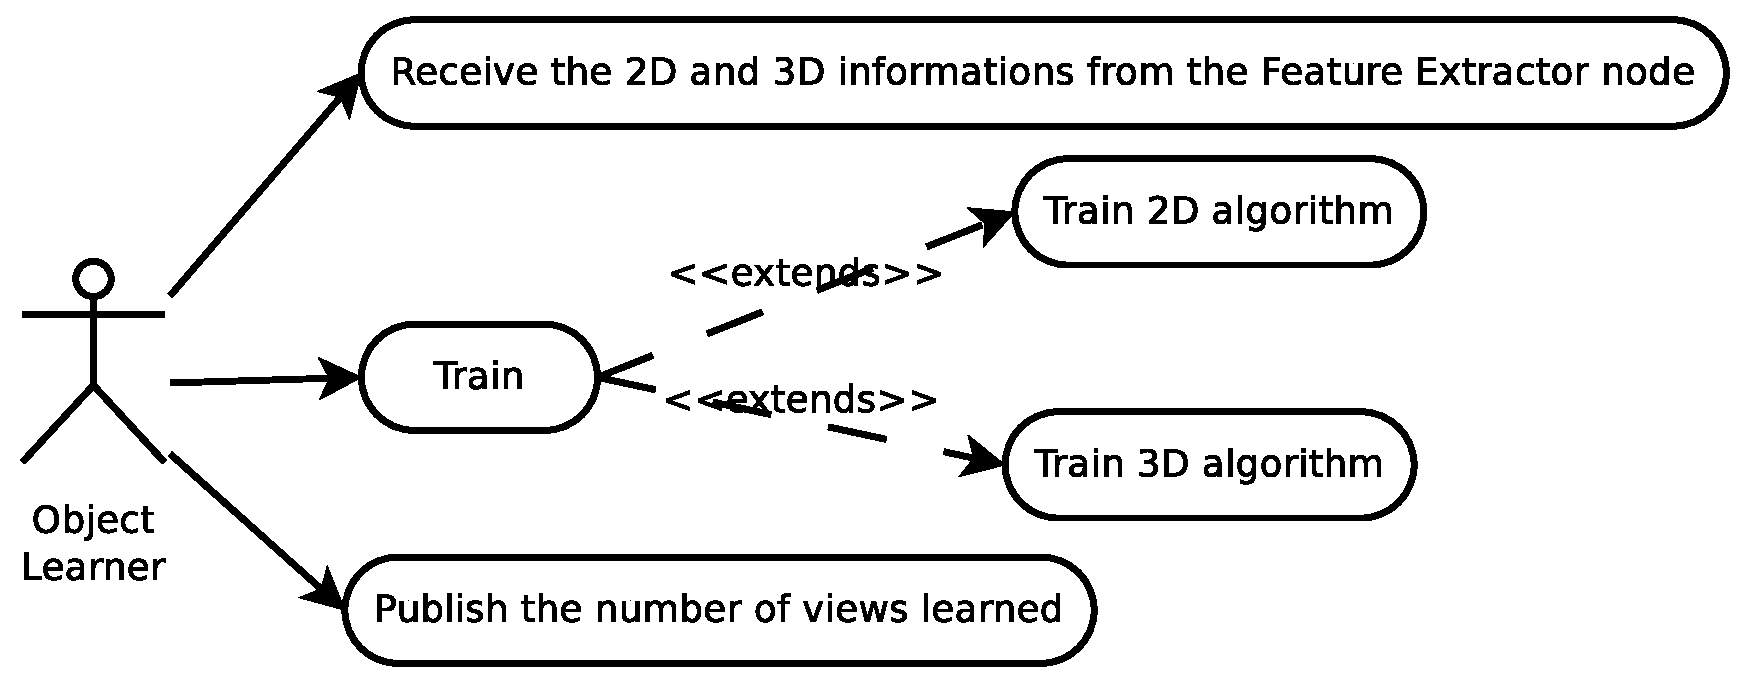
\includegraphics[scale=0.4]{../diagrams/images/uc_learner.eps}
	\end{center}

\subsubsection{Object Recognizer Node} 
\hspace{0.5cm}This node will track the user's hands and recognize the held objects. 

There are two different algorithms, one trained with the 2D data and the other one trained with the 3D data. More information about those algorithms may be found in the Functional Requirements section. 
\\
The steps done by this node are the following: 
First, as in the Learning Mode, 2D and 3D descriptors will be extracted. Then, the algorithms will compare that information with the learned one. 
The output of each algorithm will be a percentage of similarity between the dataset and the new object. 
\\
The 3D information is more reliable than the 2D. The latter is subjected to inaccuracies due to illumination or view angle that affects the descriptors extracted and hence the object recognition.
\\
Due to this fact, weights for the output of each algorithm will be given. Those give a higher importance to the 3D descriptors since they are more robust. 
\\
The object that is finally published in a topic will be the one with a higher percentage of similarity. 

\begin{center}
	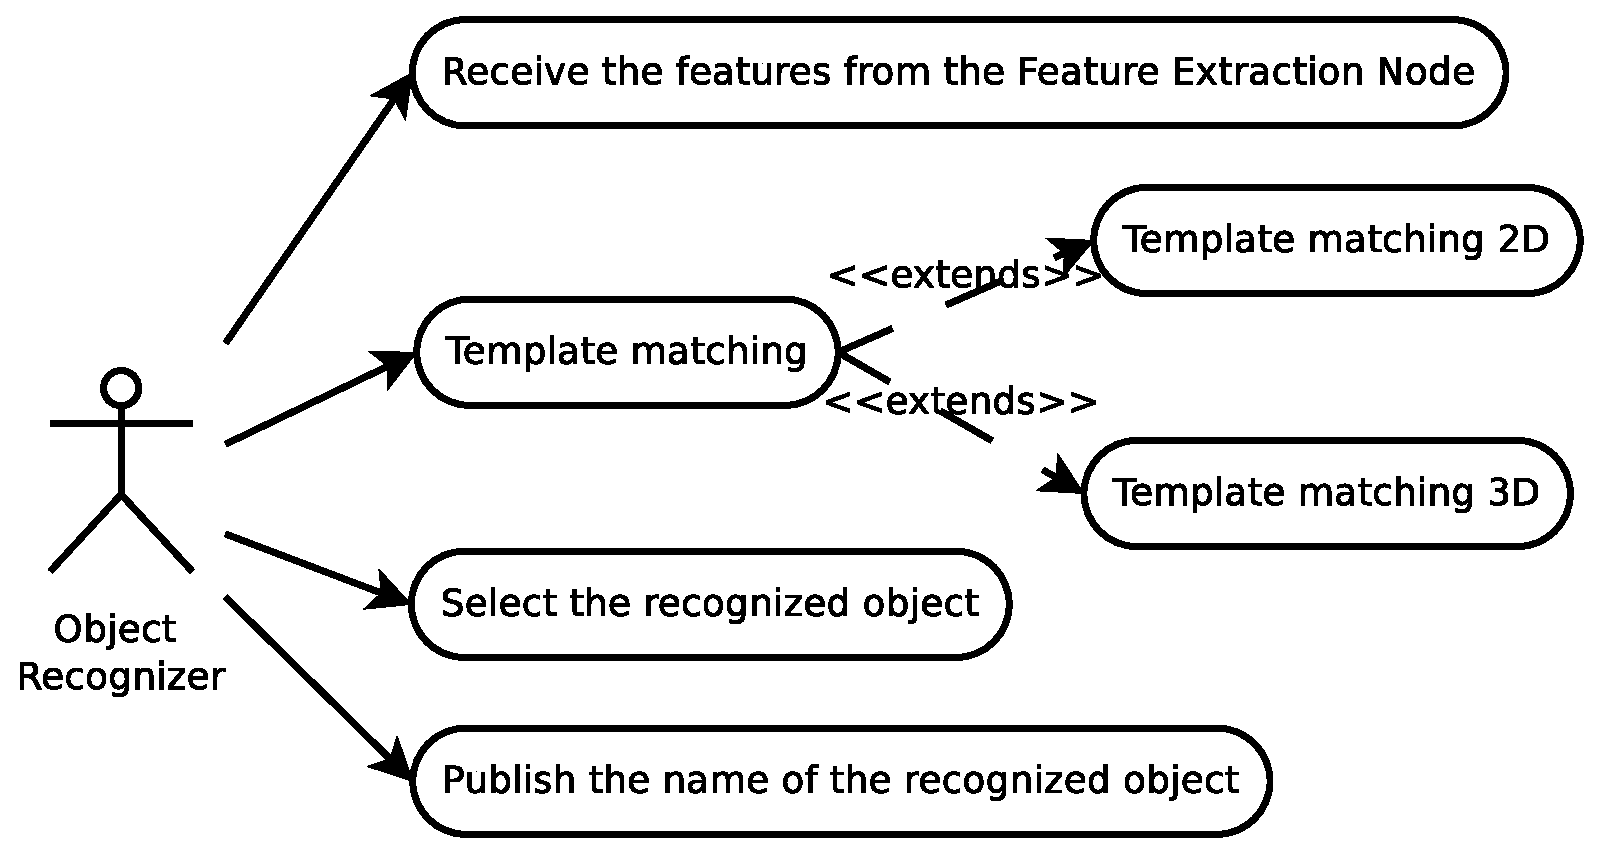
\includegraphics[scale=0.4]{../diagrams/images/uc_recognizer.eps}
\end{center}

\subsubsection{Converter Node}

This node will convert the messages from other ROS packages to the internal message format used within the code. 

\begin{center}
	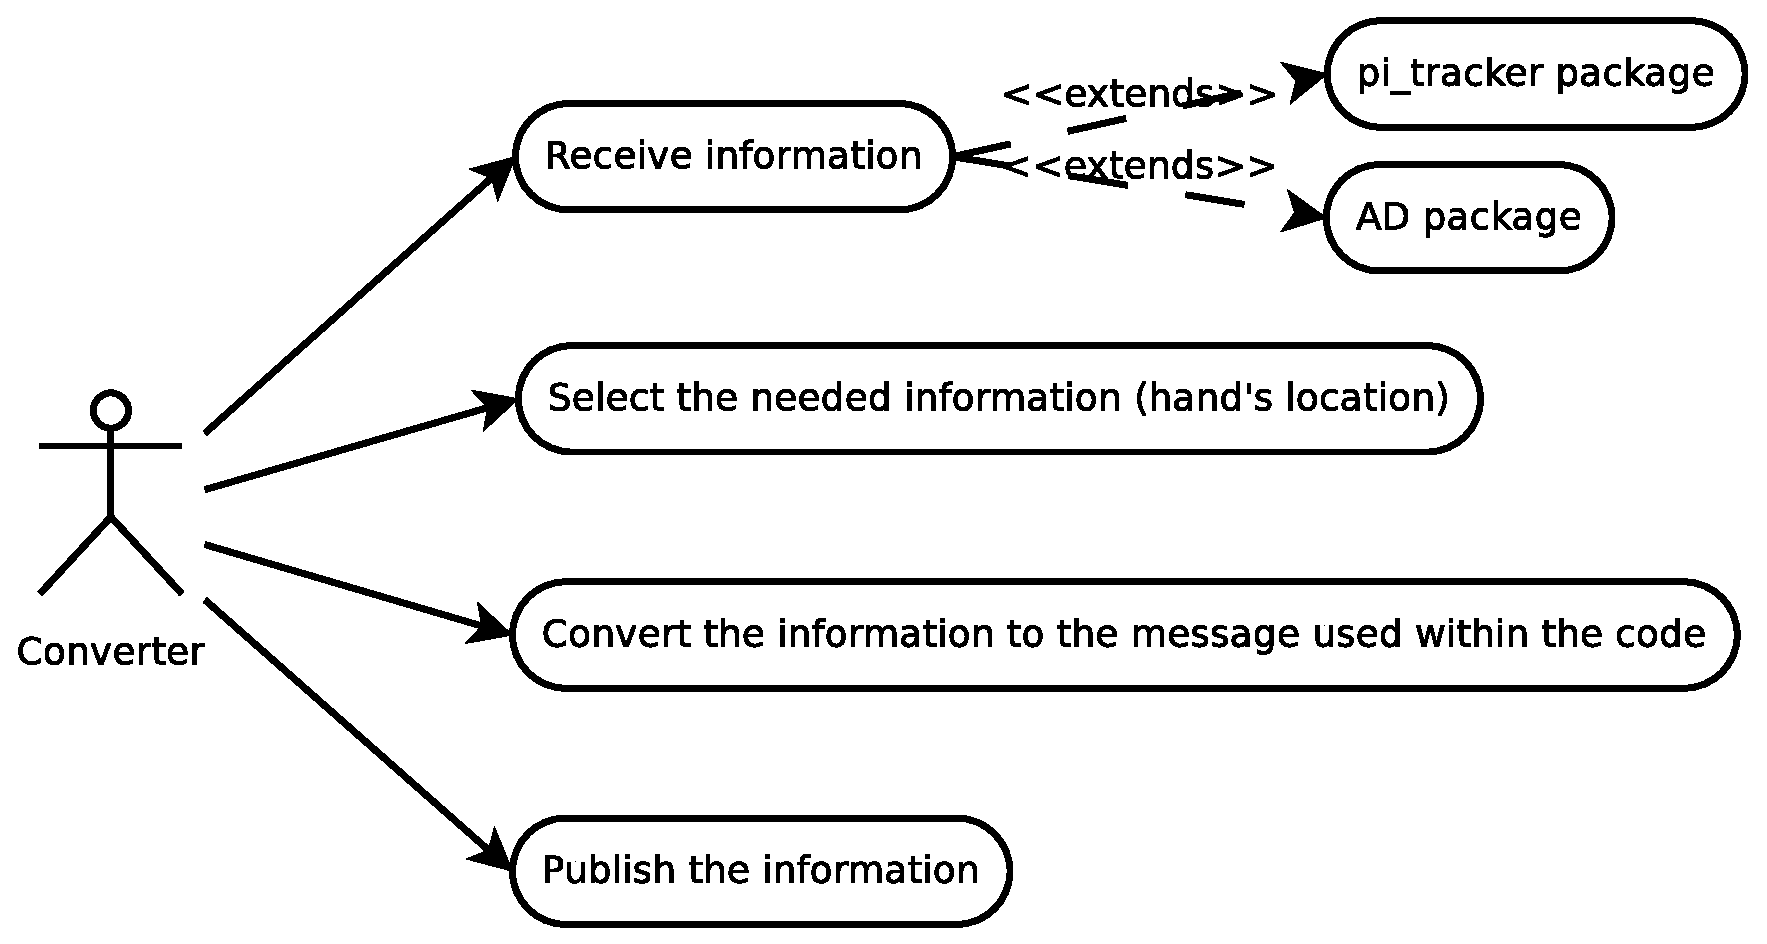
\includegraphics[scale=0.4]{../diagrams/images/uc_converter.eps}
\end{center}
	
\subsubsection{ROI Segmenter Node}
This node will segment the ROI (Region Of Interest) both in 2D and 3D.

\begin{center}
	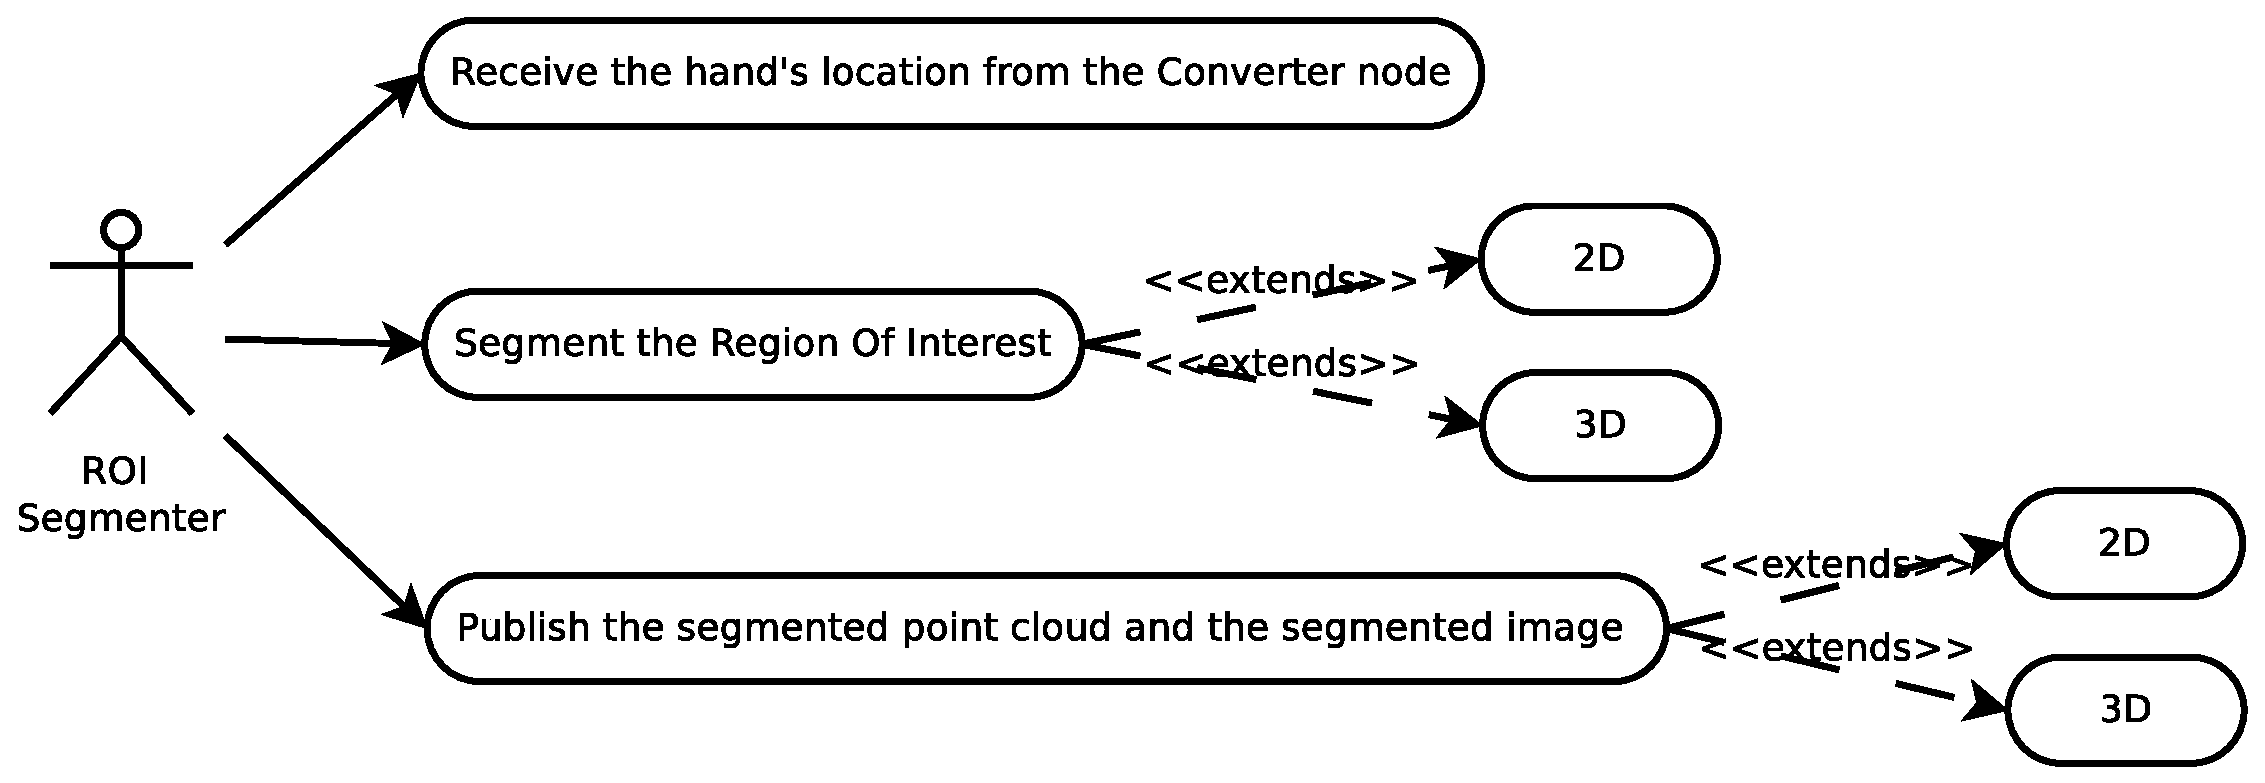
\includegraphics[scale=0.4]{../diagrams/images/uc_roi_segmenter.eps}
\end{center}

\subsubsection{Feature Extractor Node}
This node will extract both 2D and 3D features and publish them. 

\begin{center}
	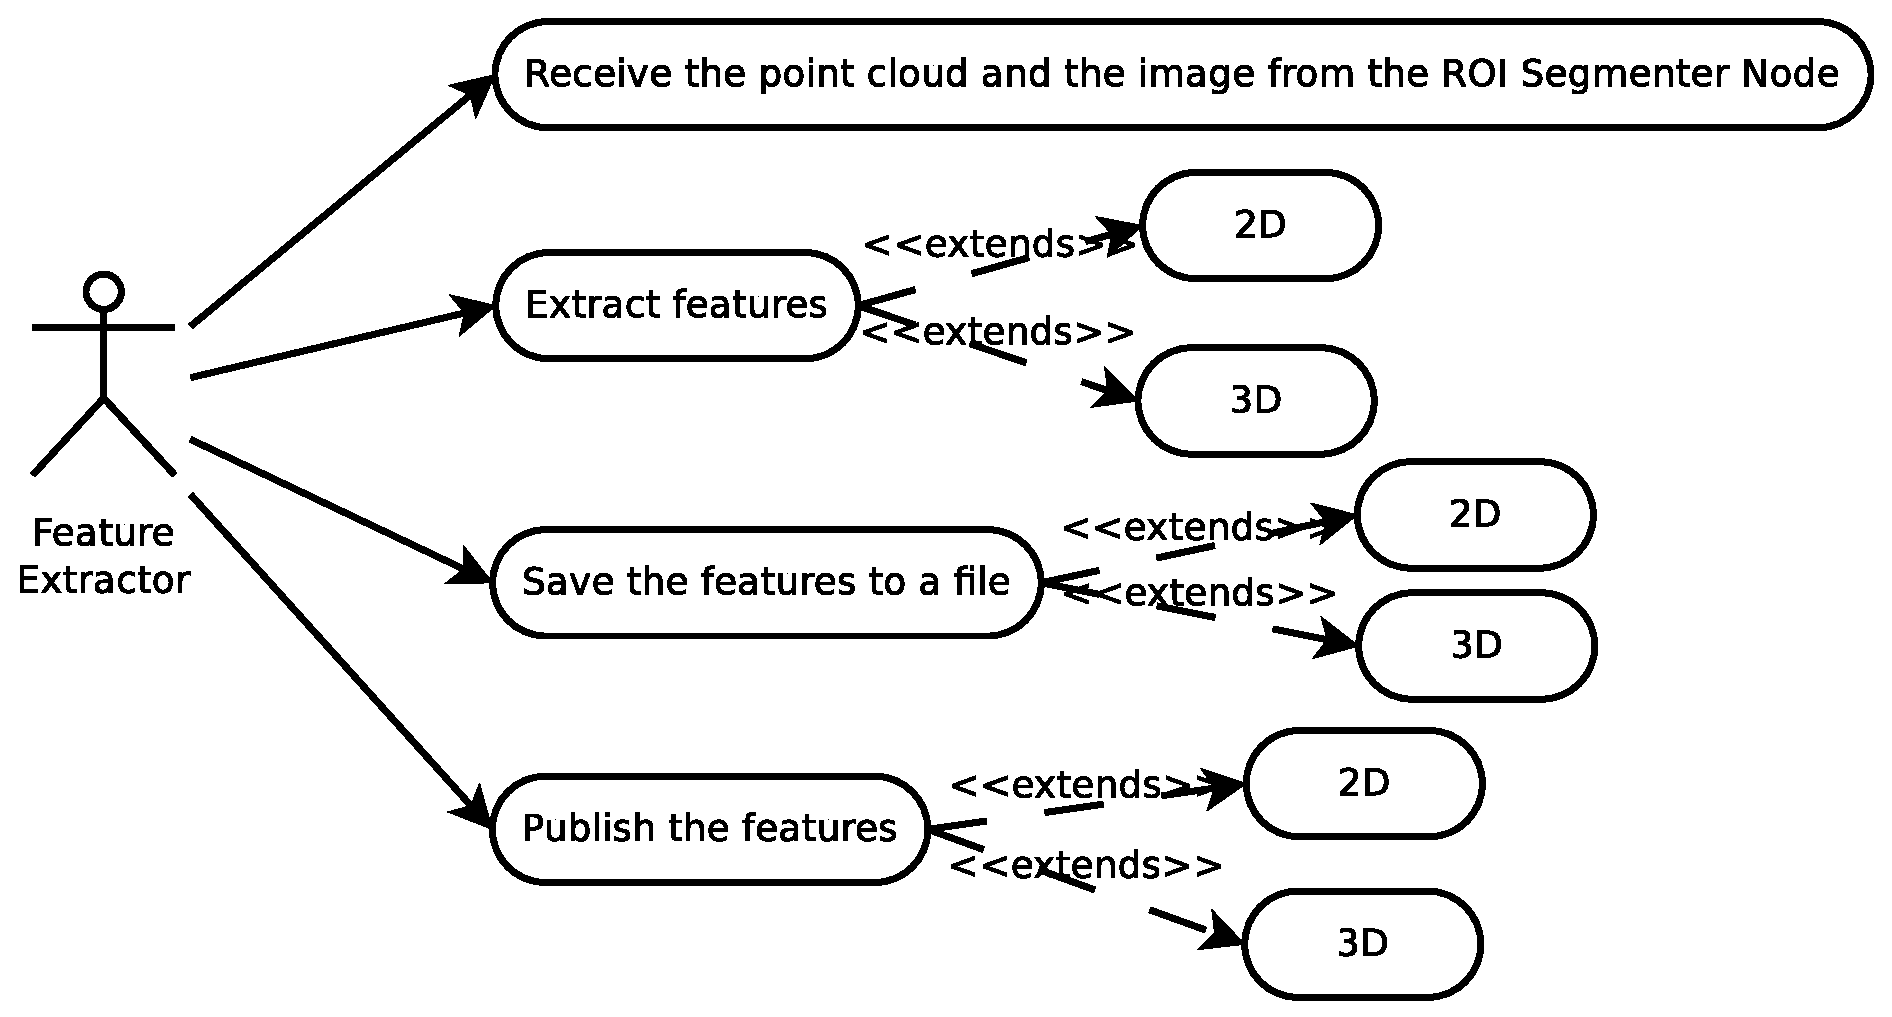
\includegraphics[scale=0.4]{../diagrams/images/uc_feature_extractor.eps}
\end{center}


\subsubsection{Data Parser Node}
This node will store the 2D and 3D features of each template of the same object in one file. 
\begin{center}
	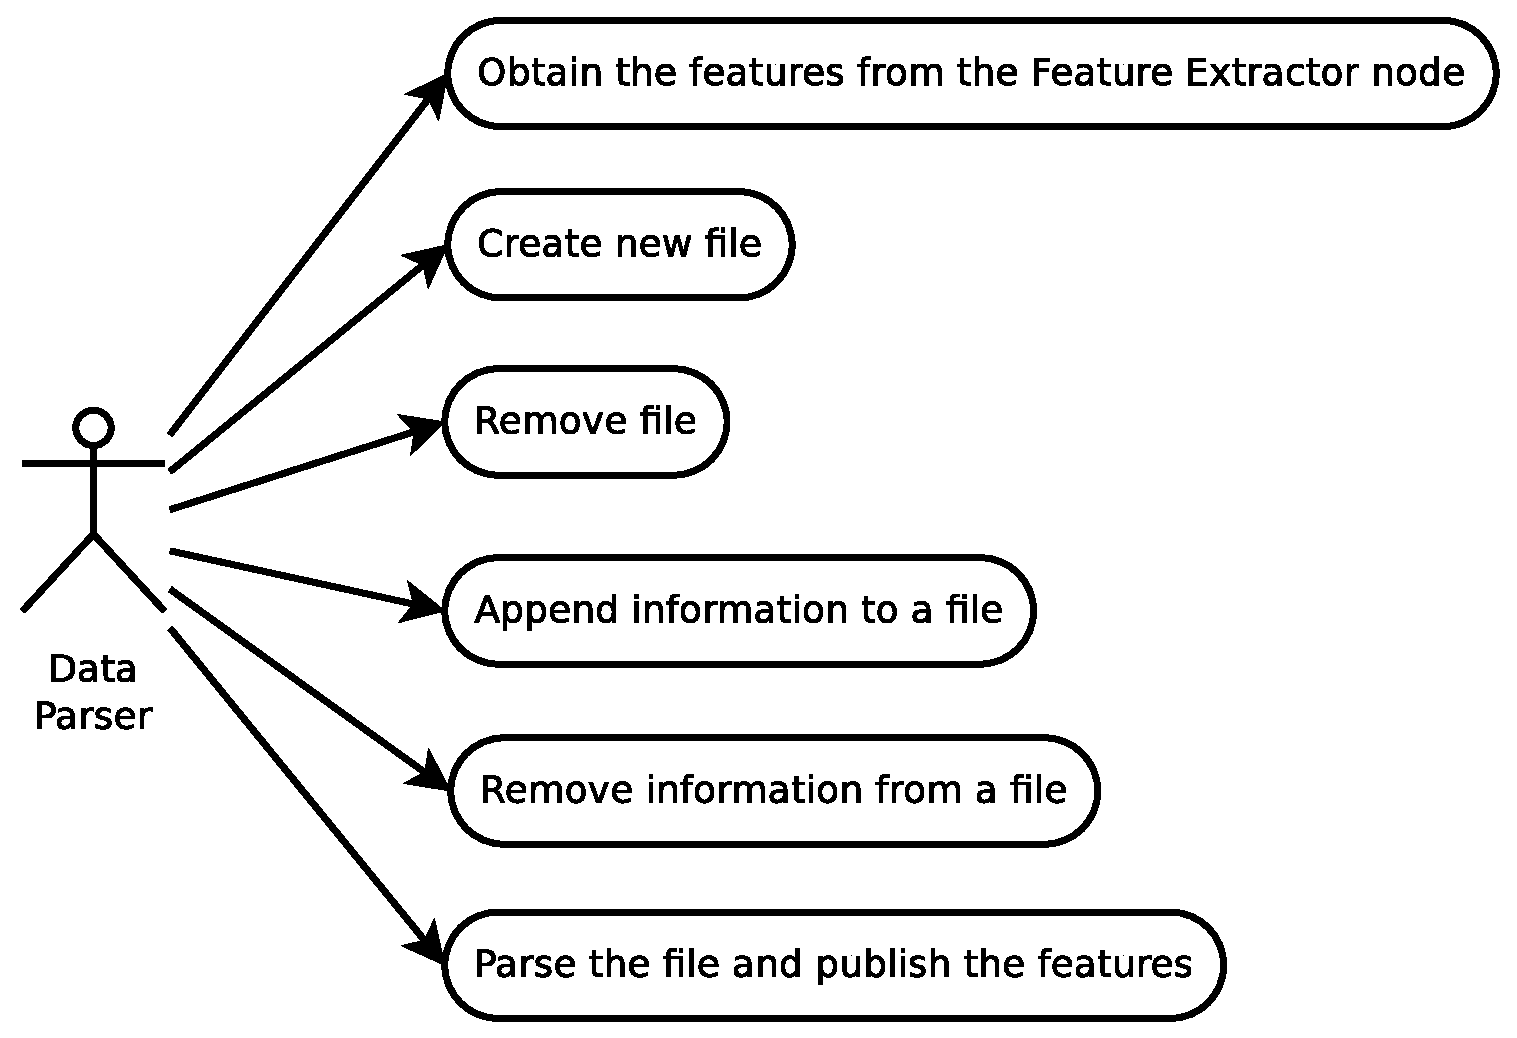
\includegraphics[scale=0.4]{../diagrams/images/uc_data_parser.eps}
\end{center}


\subsection{Third Party Packages}
\hspace{0.5cm}Initially only one third party ROS package will be used, to track the hand's position: pi\_ tracker. This software publishes the hand's position and there will a node in the proposed software (Conversion Node, whose requirements are specified in the next section) that converts the information returned by pi\_ tracker to the custom message used in the rest of the code.  

\subsection{Node Interaction}
%In the following diagram it can be seen the interaction and the information exchanged between nodes.
%\subsubsection{Use Case Diagram}
%\begin{center}
%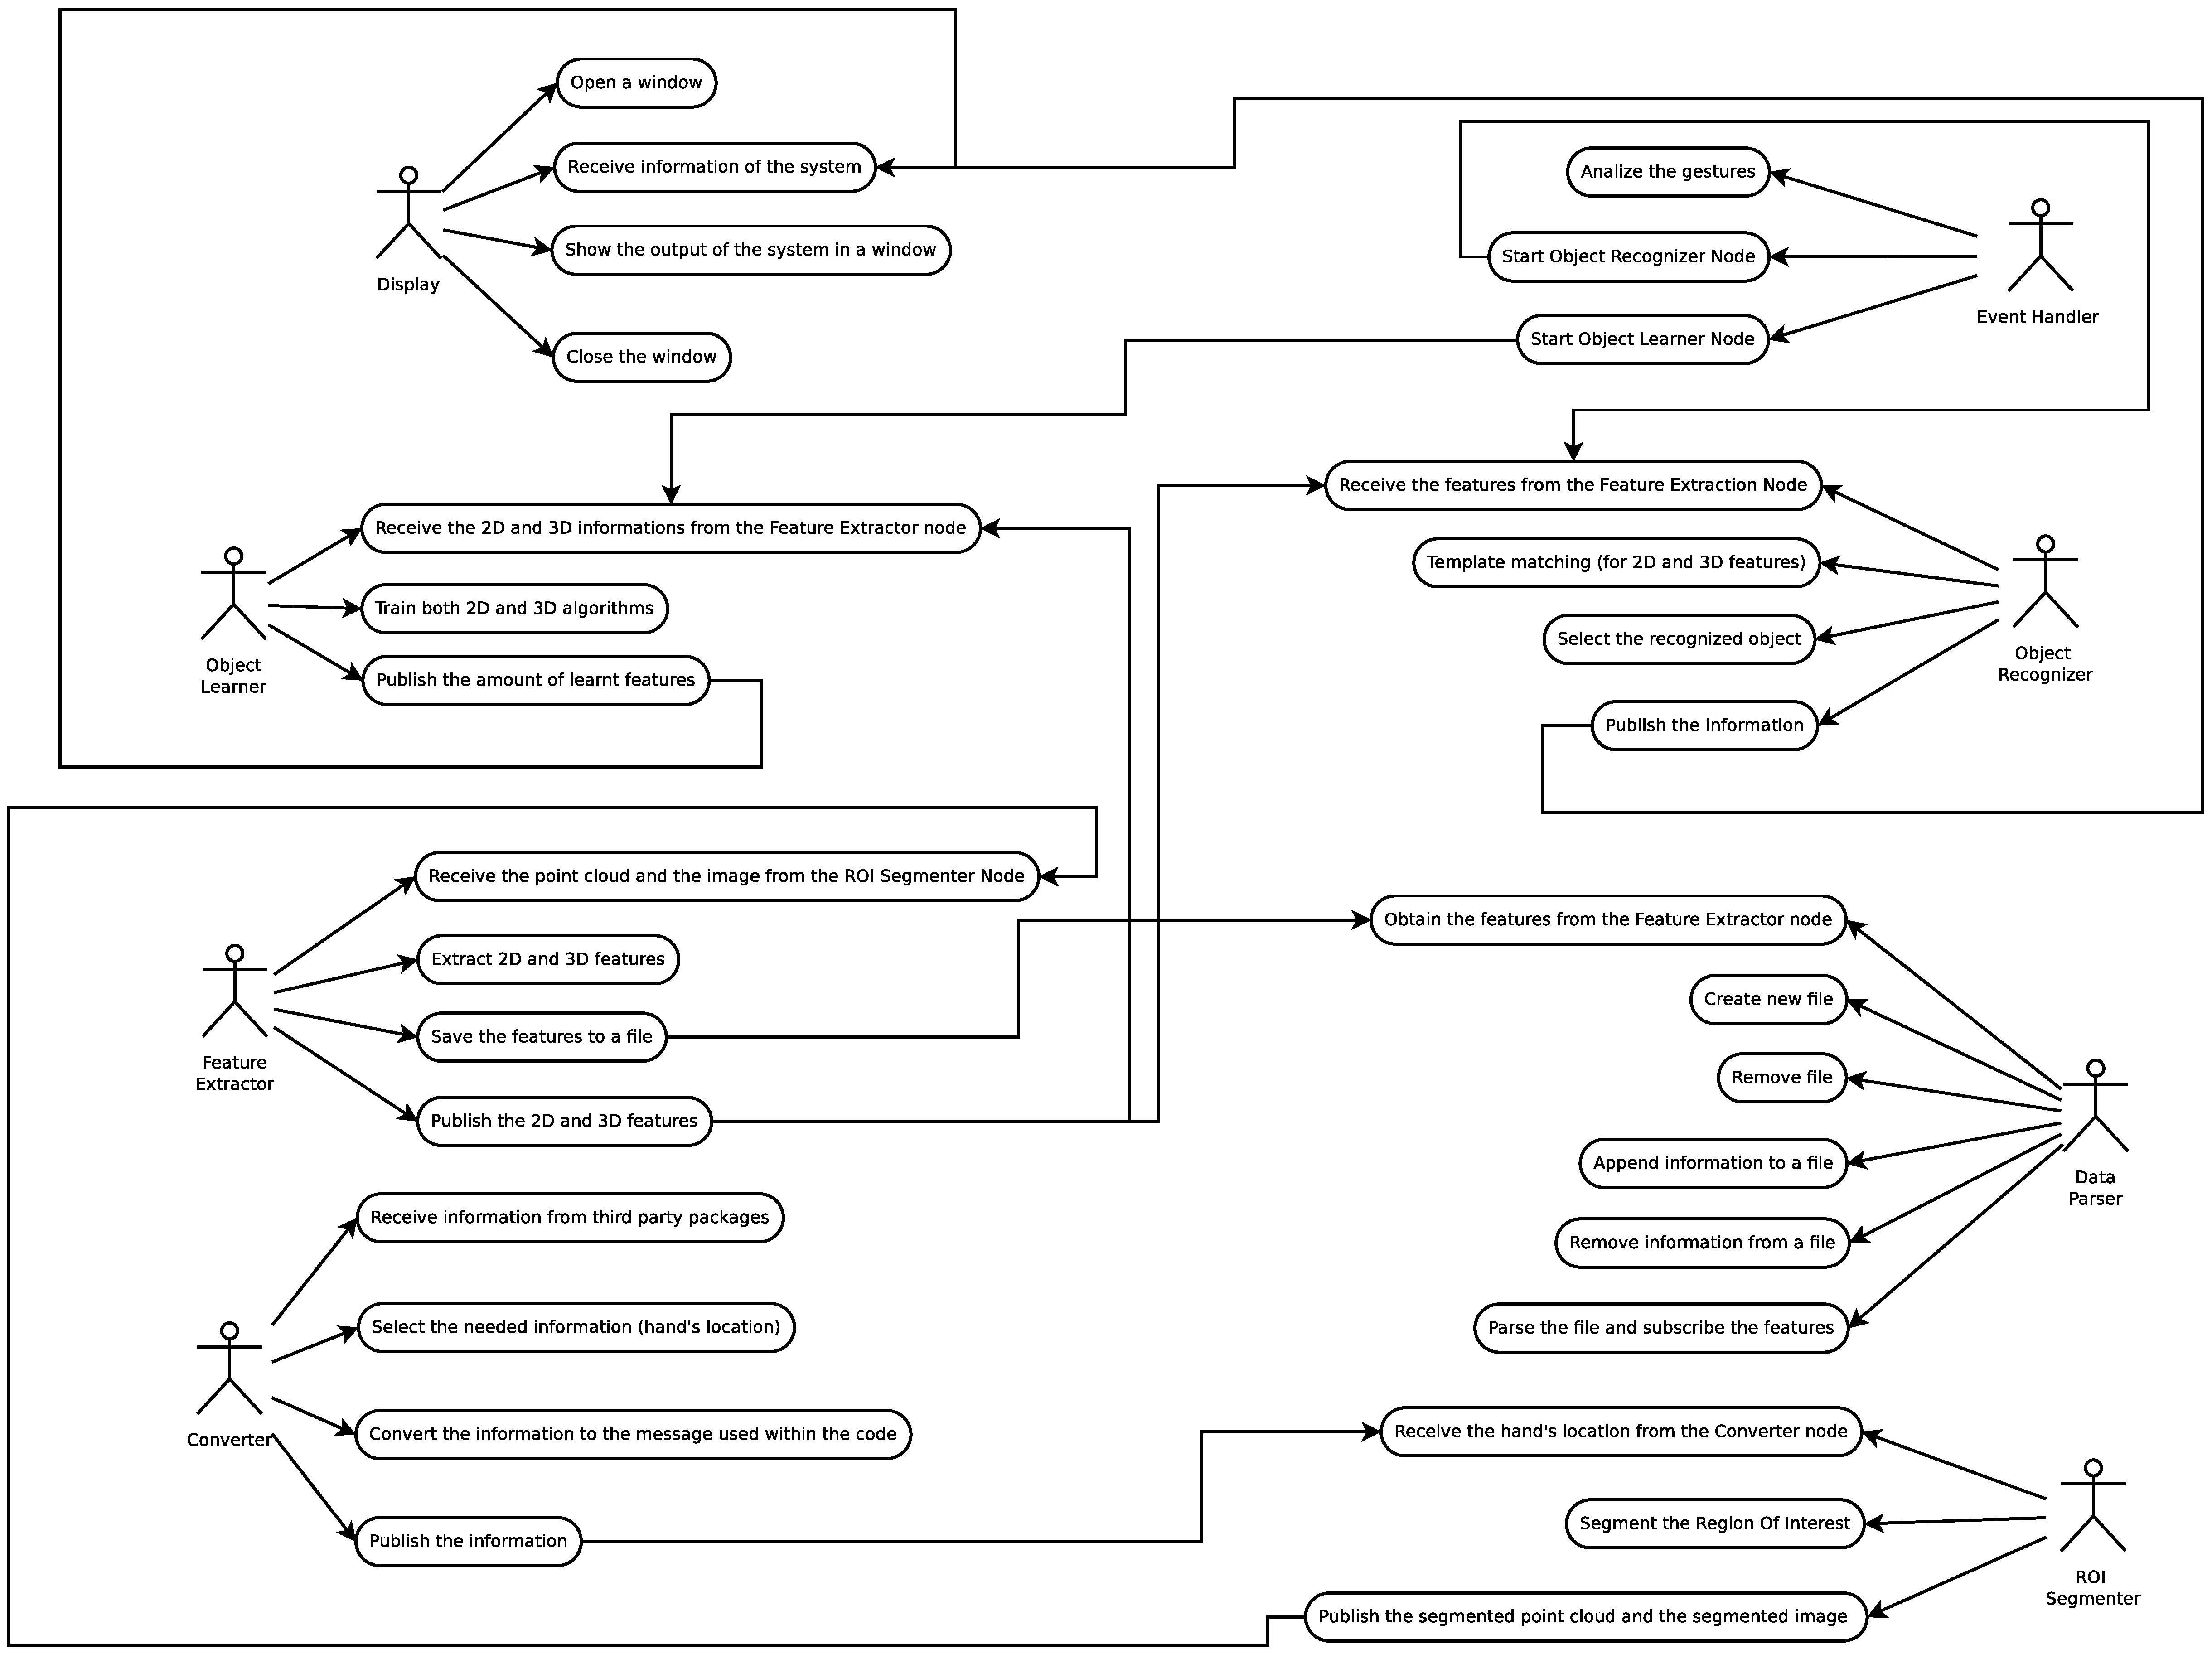
\includegraphics[scale=0.3]{../diagrams/images/use_case.eps}
%\end{center}

\subsubsection{Sequence Diagram}
In the following diagram can be seen the interaction between nodes. 
\begin{center}
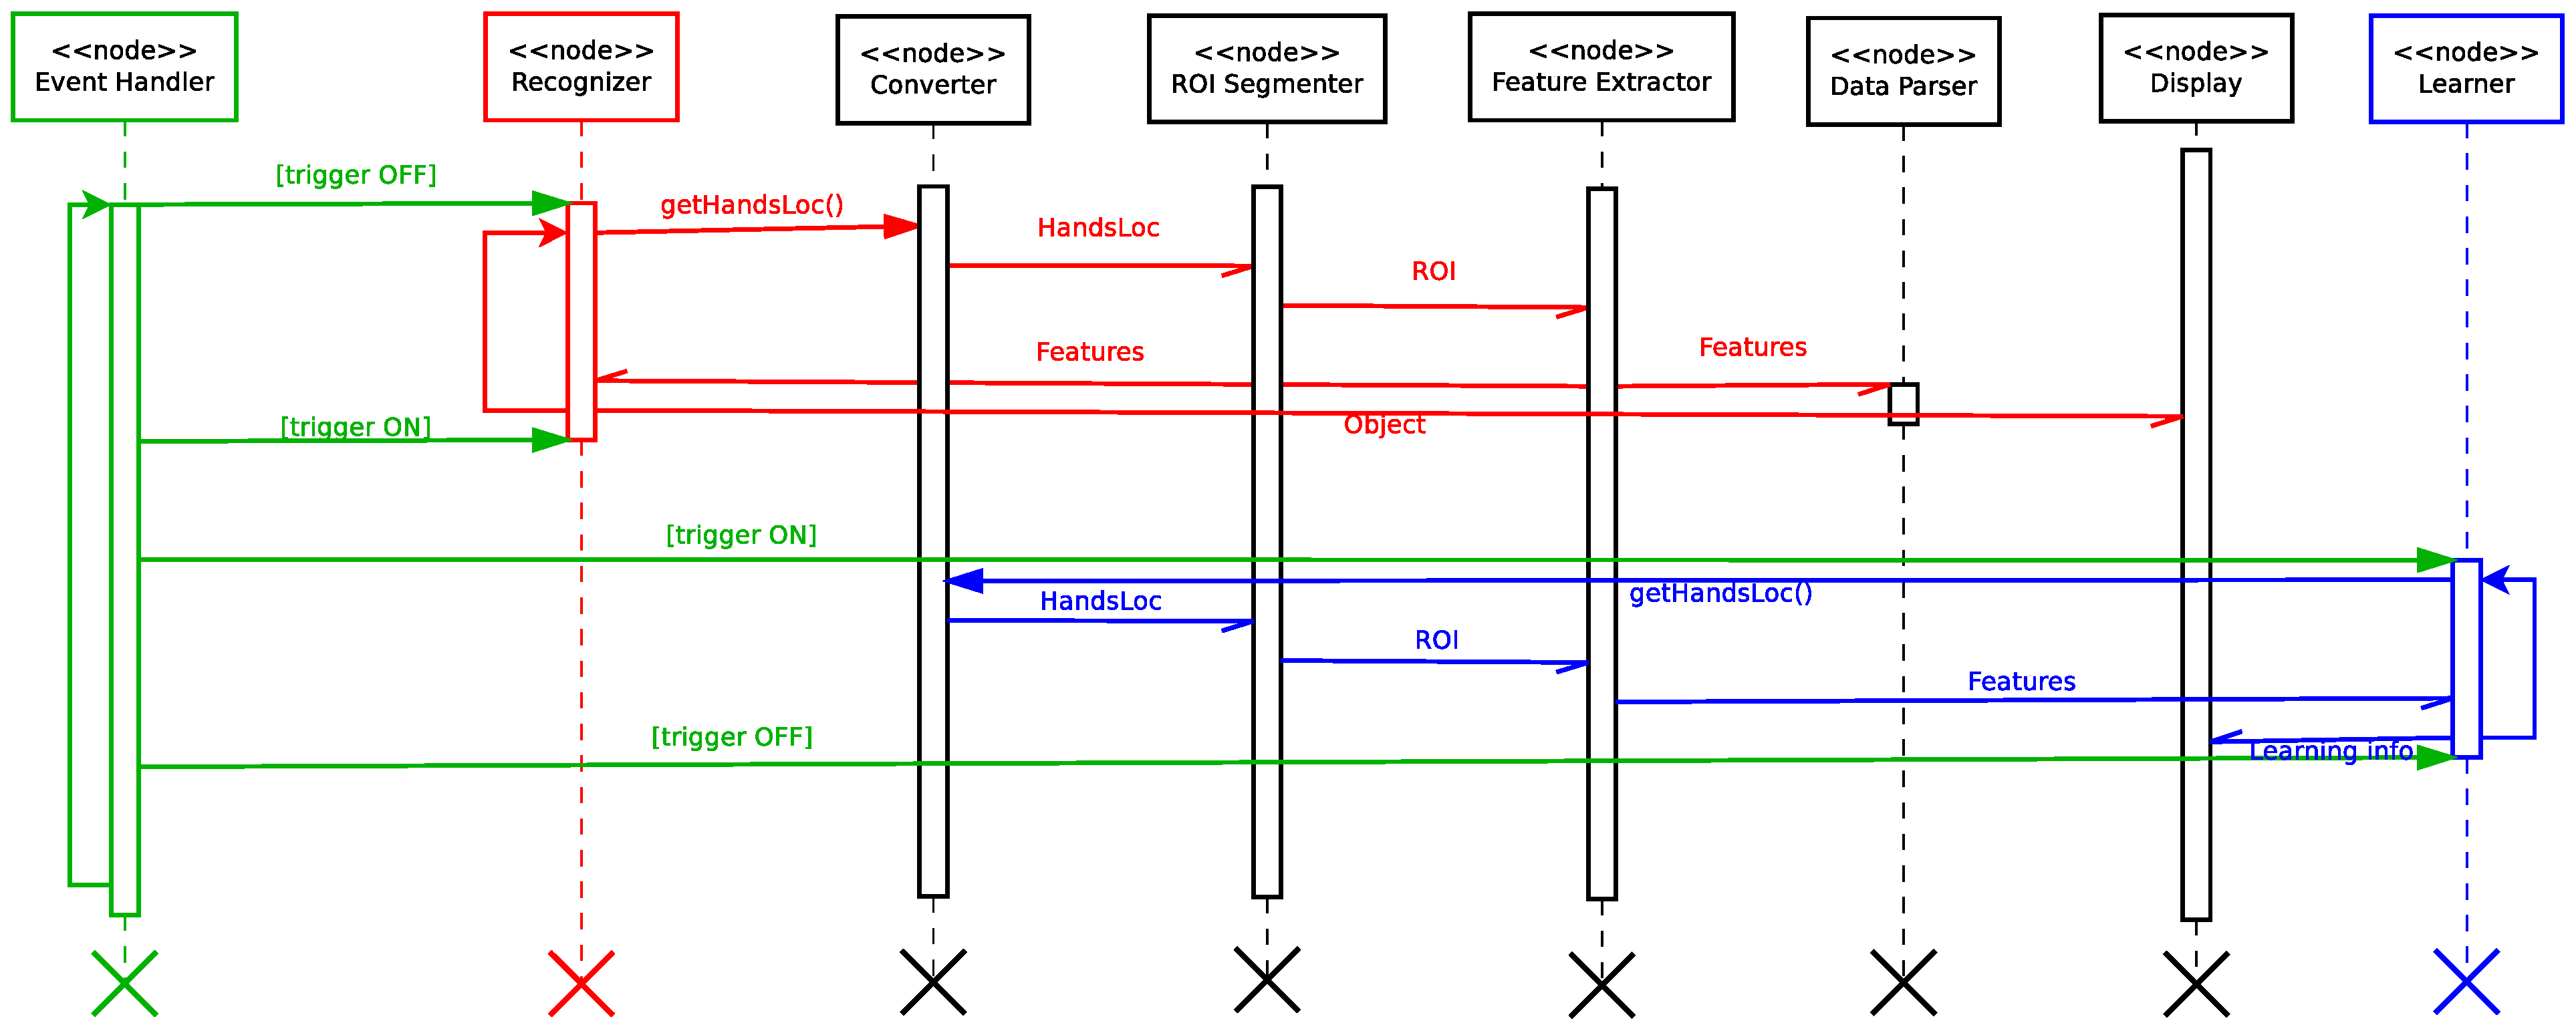
\includegraphics[scale=0.4]{../diagrams/images/sequence.eps}
\end{center}

\subsection{Flowchart}
In the following diagram, the flow of the program is represented. 
\begin{center}
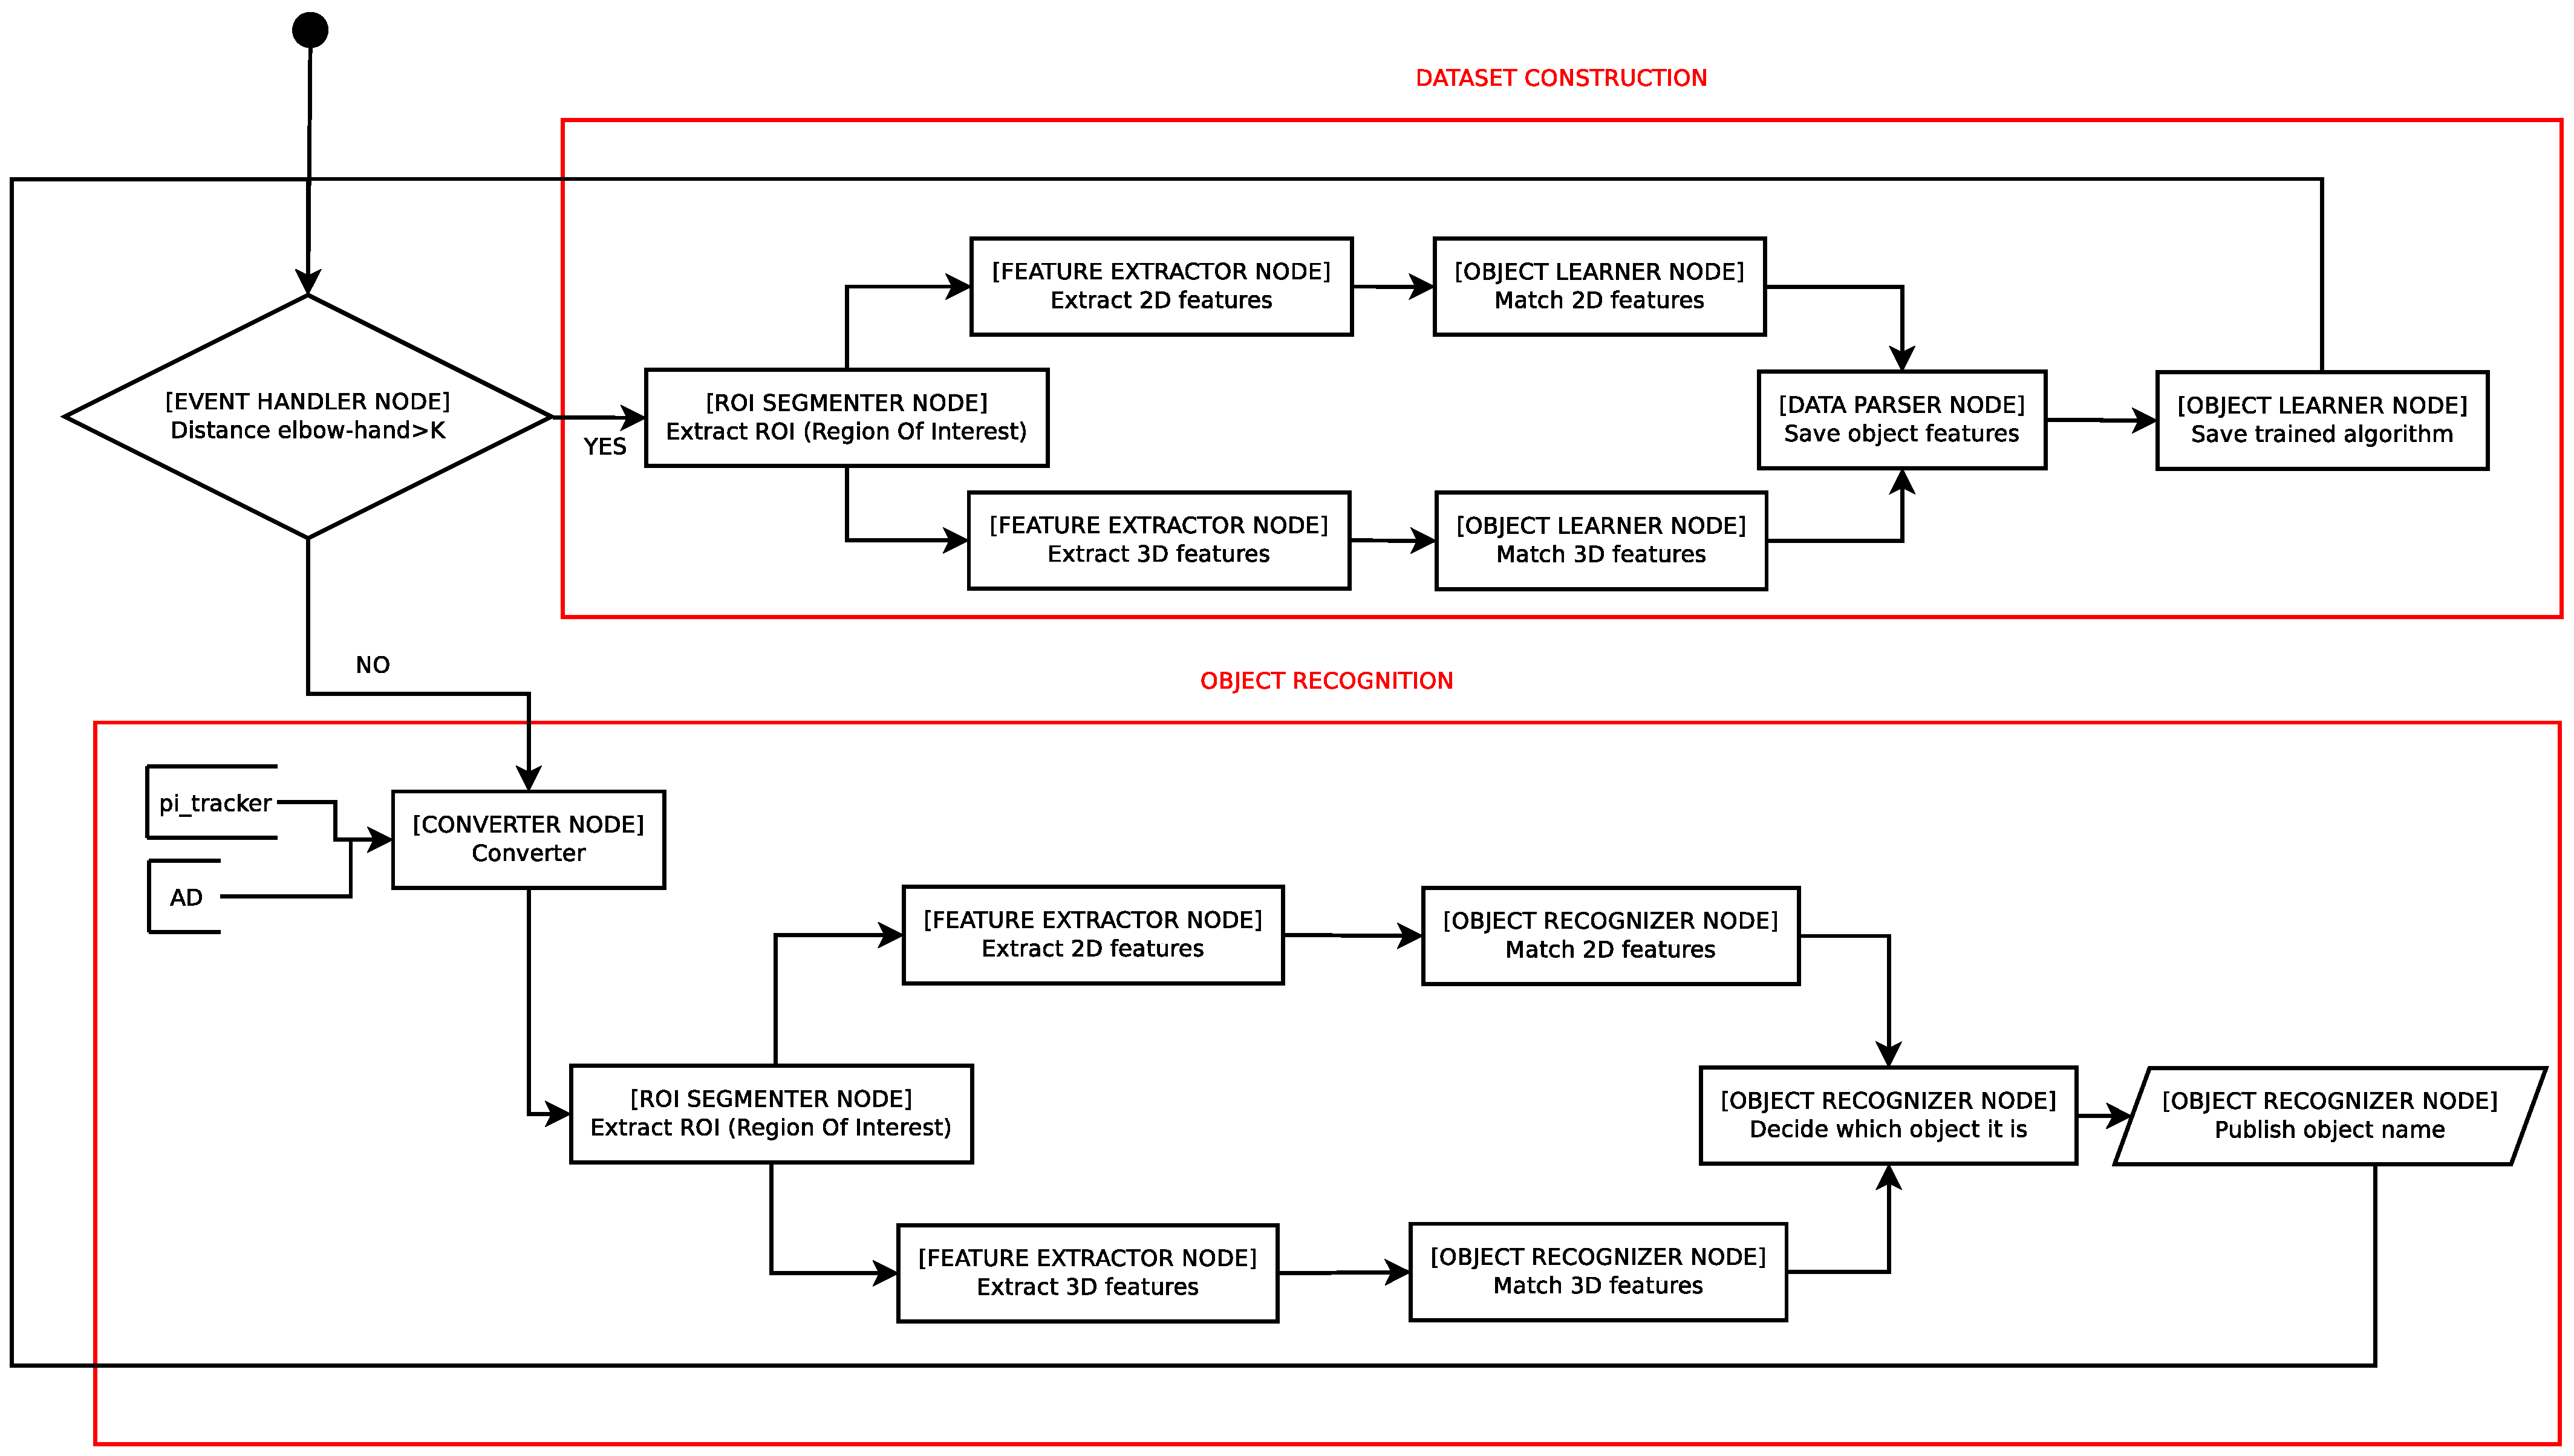
\includegraphics[scale=0.35]{../diagrams/images/flowcharts.eps}
\end{center}





\section{Functional requirements}

\subsection{General requirements}
\begin{enumerate}[label=\textbf{FR\threedigits*}, leftmargin=2cm]

	\item The software must be developed under ROS (Robotic Operating System), using the Groovy distro and rosbuild.
	\item A version control system should be used (GIT) and all the code must be periodically updated in the following github repository:  $https://github.com/irenesanznieto/TFG$
	\item The software has to have an interface. Its requirements are specified in the following "Interface Requirements" section. 
	\item The software must accept as inputs the following RGB-D sensors: Microsoft Kinect, ASUS Xtion PRO, ASUS Xtion PRO Live, PrimeSense PSDK 5.0.
	\item The output of the system must be a node specifying the name of the detected object. 
 
\subsection{Event Handler}
 
\subsection{Display}

\item The program must have one window with the output of the camera of the kinect sensor. 
\item The information as to what mode the program is in has to be shown in the title of the window.
\item In the recognition mode, the interface must show a square around the detected object and a text label indicating the object's name. Also, two points must be drawn in each of the hands. 
%\item The learning mode should open a new window where an shpere will appear. The sphere must show a different colour when a template of that zone is made. On the main window, a square should be placed around the new object. 
\item The learning mode should display the number of views obtained and processed of the object as well as an indication as to how to rotate the object to obtain further views. 


\subsection{Object Learner}
	\item The input to this node will be the features (both 2D and 3D) extracted from the feature extractor node. 
	\item This node must have two algorithms, one for 2D and other for 3D. 
	\item The algorithm used with 2D features should be a BruteForce trainer.
	\item The algorithm used with 3D features will be the Line-Mod trainer. 	
	\item This node must send feedback messages to the display with the learning information (number of views of the object processed, information about how to rotate the object).
	\item The output of this node will be the trained algorithms, whose parameters must be written to a file. 

\subsection{Object Recognizer}
	\item This node must have two algorithms, one for 2D and other for 3D. 
	\item The algorithm used with 2D features should be a BruteForce matcher.
	\item The algorithm used with 3D features will be the Line-Mod matcher. 
	\item A weighting must be made to the output of the matching process. This will help reduce the false positives and negatives by modelling occlusions depending on the hand-elbow relative positions. 
	\item A weighting must be made depending on the amount of texture possessed by each object to decide which matching should have more importance, the 2D or the 3D one. 



\subsection{Converter}

\item The information should be received subscribing to the topics of the different third-party packages. 
\item The internal message format must have the following structure: \\[0.3cm]
\textit{
std\_ msgs/Header header\\[0.1cm]
int32 id\\[0.1cm]
geometry\_ msgs/Vector3[] position\\
\hspace*{0.5cm}float64 x\\
\hspace*{0.5cm}float64 y\\
\hspace*{0.5cm}float64 z\\
}


\subsection{ROI Segmenter}
	\item This node will segment the Region Of Interest both in 2D (image) and in 3D (point cloud). 
	\item In the 3D segmentation, the ROI will be a box around the hand. 
	\item The original point cloud will be filtered using a depth filter to eliminate the background. After that, the dimensions of the box will be obtained locating the maximum and minimum points in the x, y and z axis. 
	\item The size of the 2D ROI must be extracted from the 3D ROI x and y dimensions. Those measures will be transformed to pixels. 
	\item The 2D ROI will be cropped from the original image using the points obtained from the 3D ROI. 

\subsection{Feature Extractor}
\item This node will extract both 3D and 2D features. 
\item The 2D features will be expressed as a vector of descriptors, using the ORB approach. 
\item The 3D features will be expressed as a vector of features, using the Line-Mod approach.

\item The 2D and 3D features of all the views of each object will be stored in a file, using the data parser node.  

\subsection{Data Parser}
\item This node will compress the features obtained to have one data file per object with all the information.
 
\item It has to be able to create a new file for storing the features of a new object. 
\item It has to be able to delete certain views or a complete file of the dataset. 
\item It has to be able to add another view to a previously stored object. 

\item This node will also be able to read the files to extract the 2D and 3D features of each object of the dataset. 

\item The name of the file will be the one given to the object. 

\item The datafile structure will be: \\
		\begin{lstlisting}
	<view1>
		<2D>
			[descriptor information ..]
		</2D>
		<3D>
			[template information ..]
		</3D>
	</view1>	
	...
	...
	...		
			
	<viewN>
		<2D>
			[descriptor information ..]
		</2D>
		<3D>
			[template information ..]
		</3D>
	</viewN>	
		
		\end{lstlisting}
	


\end{enumerate}





\section{Performance requirements}

\begin{enumerate}[label=\textbf{PR\threedigits*}]
\item The recognition must run on the lowest amount of time possible, to allow a fluid human-robot interaction. This time must be lower than 500 ms. 
\item The learning must run on the lowest amount of time possible, to allow a fluid human-robot interaction. This time must be lower than 5s. 
\end{enumerate}


%\section{Operational requirements}
%\section{Resource requirements}
%\section{Verification requirements}
%\section{Acceptance testing requirements}	%This is a validation activity; did we build the right thing? Is this what the customer really needs? 

\section{Documentation requirements}
\begin{enumerate}[label=\textbf{DR\threedigits*}]
	\item The code must be completely documented, i.e. each class, class function , class member and piece of code should have comments explaining all the aspects. 
	\item The documentation will be made using Doxygen notation, through the rosdoc\_ lite 
	% $[http://wiki.ros.org/rosdoc\_lite]$ 
	ROS package. 
	\item All the documentation must be available at the git repository. 
\end{enumerate}

%\section{Security requirements}
%\section{Portability requirements}
%\section{Quality requirements}
%\section{Reliability requirements}
\section{Maintainability requirements}
\begin{enumerate}[label=\textbf{MR\threedigits*}]
	\item The code must be as modular as possible. 
	\item All the classes' variables that are susceptible of being modified through a inheritance will be declared as protected. 
	\item Gtests will be built to demonstrate each functional requirement. 
	
\end{enumerate}

%\section{Safety requirements}

%\section{Time Schedule}


\end{document}



	
	\section{Appendix: Budget}
		This appendix presents the estimated budget of the project. 
		Appendix \ref{project_management} explained the time management followed in this project and the different phases it underwent. 
		Figure \ref{phases} shows the summary of the days spent in each of the phases. 
		The phase that occupied most of the time was the learning phase. 
		The state of the art learning occupies most of the project since it was performed in parallel with most of the other phases, as can be seen in figure \ref{gantt_diagram}. 
		The next phase in size is the project programming and then the documentation of the project. 
		% \begin{figure}[H]
		% 	\centering
		%     \includegraphics[width=0.8\linewidth]{img/budget/phases.png}
		% 	\caption[Days and hours per project phase]{Summary of the days and hours spent in each of the project's phases}	
		% 		    \label{phases}
		% \end{figure}
		\\

		It can be seen from figure \ref{phases} that the total days spent in the development of this project were 454. 
		It was assumed that around 60 days between the begin and end dates were not devoted to this thesis. 
		Also, an average of 3 hours per day were reserved to implementing this system and hence the total hours used were 1362. 
		% The man hours performed by my advisor were calculated as one hour per week as average. 
		Figure \ref{budget} shows the final budget of the project. 
		The first two items are the hardware required, then the man hours cost and finally the software cost. 
		It can be noted that the software total cost was of 0 \euro. 
		This is because all software used in this system is Open Source, hence no licenses were paid. 


		% \begin{figure}[H]
		% 	\centering
		%     \includegraphics[width=0.8\linewidth]{img/budget/budget.png}
		% 	\caption[Project's budget]{Project's budget}	
		%     \label{budget}
		% \end{figure}

\begin{table}[H]
\centering
\begin{tabular} {l c c c c}
\toprule
\addlinespace[3mm]
   \multicolumn{1}{c}{\begin{center}\textbf{ITEM}\end{center}} &
   \multicolumn{1}{c}{\begin{center}\textbf{COST (\euro)}\end{center}} &
   \multicolumn{1}{c}{\begin{center}\textbf{UNITS}\end{center}} &
   \multicolumn{1}{c}{\begin{center}\textbf{QUANTITY}\end{center}} &
   \multicolumn{1}{c}{\begin{center}\textbf{TOTAL COST (\euro)}\end{center}} &
\\
\addlinespace[-3mm]
\midrule
\textbf{Hardware}	&&&&		\\					
\hspace*{0.5cm}	Kinect 360	&	120	&	\euro/unit	&	1 	&	120 \\
\hspace*{0.5cm}	Mountain Ivy 11 Laptop	&	1000	&	\euro/unit	&	1	&	1000\\		
\textbf{Man hours}													&&&&		\\		
% \hspace*{0.5cm}	Senior Engineer 	&	12	&\euro/h	&	56.75	&	681\\
\hspace*{0.5cm}	Undegraduate Engineer	&	8	&	\euro/h		&	1362	&	10896 \\
						
\textbf{Software}			&&&&		\\						
						
\hspace*{0.5cm}	Linux	&	0 &	\euro/license	&	1	&	0\\
\hspace*{0.5cm}	ROS	&	0	&\euro/license&	1	&0\\
\hspace*{0.8cm}		openni\_camera	&	0	&	\euro/license	&1&		0\\
\hspace*{0.8cm}		openni\_launch	&	0	&	\euro/license	&1&	0\\
\hspace*{0.8cm}		pi\_tracker 		&	0	&	\euro/license	&1&	0\\
\hspace*{0.5cm}	PCL		&	0	&	\euro/license	&	1	&	0\\
\hspace*{0.5cm}	OpenCV	&	0	&	\euro/license	&	1	&	0\\
						
\midrule

\textbf{TOTAL PROJECT'S COST: }			&&&&			\textbf{12016}\\

\bottomrule
\end{tabular}
\caption[Project's budget]{Project's budget}
\label{budget}

\end{table}


		Since all the software used is Open Source, I have performed an estimation of the cost of the development of each of the libraries I have used in this project. 
		Figure \ref{estimations} summarizes the results.  

		% \begin{figure}[H]
		% 	\centering
		%     \includegraphics[width=0.6\linewidth]{img/budget/estimations.png}
		% 	\caption[Open source software cost estimation]{Open source software cost estimation}
		%     \label{estimations}	
		% \end{figure}





\begin{table}[H]
\centering
\begin{tabular} {l r}
\toprule
\addlinespace[3mm]
   \multicolumn{1}{c}{\begin{center}\textbf{SOFTWARE}\end{center}} &
   \multicolumn{1}{c}{\begin{center}\textbf{TOTAL COST (k\euro)}\end{center}} &
\\
\addlinespace[-3mm]
\midrule
Linux	(Ubuntu 13.04, 64 bits) &	10680%.392
	\\
ROS		(Groovy distribution, v1.9.50)&	2932%.34325	
\\
\hspace*{0.5cm}	openni\_camera	(v1.8.9)&	99%.315.98	
\\
\hspace*{0.5cm}	openni\_launch	(v1.8.3)&	6%5.95698		
\\
\hspace*{0.5cm}	pi\_tracker 	(Groovy release)&	74%09269	
\\
PCL	(v1.7.1)	&	13101%.526.72		
\\
OpenCV	(v2.3.1)	&	36264	%36263862.04		
\\
OCULAR	&	59 	%58.709439
	\\
\midrule

\textbf{TOTAL ESTIMATED COST: } & \textbf{63216}\\

\bottomrule
\end{tabular}
\caption[Open source software cost estimation]{Open source software cost estimation}
\label{estimations}

\end{table}


		The estimations are created using the SLOCCount Open Source program \cite{sloccount}. 
		This software measures the number of lines and automatically estimates the effort, time and money needed to create the software. 
		The figures in table \ref{estimations} are obtained using the basic COnstructive COst MOdel (COCOMO model) \cite{Boehm}. 
		All defaults were used and the final cost of developing each of the tools are the ones presented in figure \ref{estimations}. 
		It is important to note that in the case that these projects would not have been Open Source the cost of using them would not be, of course, the cost of the complete development. 
		Instead, a payment of a license is needed in order to obtain the right to use of the software. 
		\\

		The cost estimation of the system developed in this thesis was also performed. 
		It can be seen the high difference between the real cost and the estimated one. 
		This is mainly due to the difference in the man-hours cost. 
		By default, the software assumes a yearly cost per man of around 56 k USD which means an hourly rate of around 20 USD per hour, or 15 \euro. 
		The final cost of the developed thesis is less than 13000 \euro, including all the required hardware. 



\end{appendices}


\end{document}




%state of the art: explain the differences between previous methods and the current one. 
%---> the sift surf descr in system description
%Methods--> experiments description 
% add part: System Description -------------> DONE

